\documentclass[]{book}
\usepackage{lmodern}
\usepackage{amssymb,amsmath}
\usepackage{ifxetex,ifluatex}
\usepackage{fixltx2e} % provides \textsubscript
\ifnum 0\ifxetex 1\fi\ifluatex 1\fi=0 % if pdftex
  \usepackage[T1]{fontenc}
  \usepackage[utf8]{inputenc}
\else % if luatex or xelatex
  \ifxetex
    \usepackage{mathspec}
  \else
    \usepackage{fontspec}
  \fi
  \defaultfontfeatures{Ligatures=TeX,Scale=MatchLowercase}
\fi
% use upquote if available, for straight quotes in verbatim environments
\IfFileExists{upquote.sty}{\usepackage{upquote}}{}
% use microtype if available
\IfFileExists{microtype.sty}{%
\usepackage{microtype}
\UseMicrotypeSet[protrusion]{basicmath} % disable protrusion for tt fonts
}{}
\usepackage[margin=1in]{geometry}
\usepackage{hyperref}
\hypersetup{unicode=true,
            pdftitle={Do not use averages with Likert scale data},
            pdfauthor={Dwight Barry},
            pdfborder={0 0 0},
            breaklinks=true}
\urlstyle{same}  % don't use monospace font for urls
\usepackage{natbib}
\bibliographystyle{plainnat}
\usepackage{color}
\usepackage{fancyvrb}
\newcommand{\VerbBar}{|}
\newcommand{\VERB}{\Verb[commandchars=\\\{\}]}
\DefineVerbatimEnvironment{Highlighting}{Verbatim}{commandchars=\\\{\}}
% Add ',fontsize=\small' for more characters per line
\usepackage{framed}
\definecolor{shadecolor}{RGB}{248,248,248}
\newenvironment{Shaded}{\begin{snugshade}}{\end{snugshade}}
\newcommand{\KeywordTok}[1]{\textcolor[rgb]{0.13,0.29,0.53}{\textbf{{#1}}}}
\newcommand{\DataTypeTok}[1]{\textcolor[rgb]{0.13,0.29,0.53}{{#1}}}
\newcommand{\DecValTok}[1]{\textcolor[rgb]{0.00,0.00,0.81}{{#1}}}
\newcommand{\BaseNTok}[1]{\textcolor[rgb]{0.00,0.00,0.81}{{#1}}}
\newcommand{\FloatTok}[1]{\textcolor[rgb]{0.00,0.00,0.81}{{#1}}}
\newcommand{\ConstantTok}[1]{\textcolor[rgb]{0.00,0.00,0.00}{{#1}}}
\newcommand{\CharTok}[1]{\textcolor[rgb]{0.31,0.60,0.02}{{#1}}}
\newcommand{\SpecialCharTok}[1]{\textcolor[rgb]{0.00,0.00,0.00}{{#1}}}
\newcommand{\StringTok}[1]{\textcolor[rgb]{0.31,0.60,0.02}{{#1}}}
\newcommand{\VerbatimStringTok}[1]{\textcolor[rgb]{0.31,0.60,0.02}{{#1}}}
\newcommand{\SpecialStringTok}[1]{\textcolor[rgb]{0.31,0.60,0.02}{{#1}}}
\newcommand{\ImportTok}[1]{{#1}}
\newcommand{\CommentTok}[1]{\textcolor[rgb]{0.56,0.35,0.01}{\textit{{#1}}}}
\newcommand{\DocumentationTok}[1]{\textcolor[rgb]{0.56,0.35,0.01}{\textbf{\textit{{#1}}}}}
\newcommand{\AnnotationTok}[1]{\textcolor[rgb]{0.56,0.35,0.01}{\textbf{\textit{{#1}}}}}
\newcommand{\CommentVarTok}[1]{\textcolor[rgb]{0.56,0.35,0.01}{\textbf{\textit{{#1}}}}}
\newcommand{\OtherTok}[1]{\textcolor[rgb]{0.56,0.35,0.01}{{#1}}}
\newcommand{\FunctionTok}[1]{\textcolor[rgb]{0.00,0.00,0.00}{{#1}}}
\newcommand{\VariableTok}[1]{\textcolor[rgb]{0.00,0.00,0.00}{{#1}}}
\newcommand{\ControlFlowTok}[1]{\textcolor[rgb]{0.13,0.29,0.53}{\textbf{{#1}}}}
\newcommand{\OperatorTok}[1]{\textcolor[rgb]{0.81,0.36,0.00}{\textbf{{#1}}}}
\newcommand{\BuiltInTok}[1]{{#1}}
\newcommand{\ExtensionTok}[1]{{#1}}
\newcommand{\PreprocessorTok}[1]{\textcolor[rgb]{0.56,0.35,0.01}{\textit{{#1}}}}
\newcommand{\AttributeTok}[1]{\textcolor[rgb]{0.77,0.63,0.00}{{#1}}}
\newcommand{\RegionMarkerTok}[1]{{#1}}
\newcommand{\InformationTok}[1]{\textcolor[rgb]{0.56,0.35,0.01}{\textbf{\textit{{#1}}}}}
\newcommand{\WarningTok}[1]{\textcolor[rgb]{0.56,0.35,0.01}{\textbf{\textit{{#1}}}}}
\newcommand{\AlertTok}[1]{\textcolor[rgb]{0.94,0.16,0.16}{{#1}}}
\newcommand{\ErrorTok}[1]{\textcolor[rgb]{0.64,0.00,0.00}{\textbf{{#1}}}}
\newcommand{\NormalTok}[1]{{#1}}
\usepackage{longtable,booktabs}
\usepackage{graphicx,grffile}
\makeatletter
\def\maxwidth{\ifdim\Gin@nat@width>\linewidth\linewidth\else\Gin@nat@width\fi}
\def\maxheight{\ifdim\Gin@nat@height>\textheight\textheight\else\Gin@nat@height\fi}
\makeatother
% Scale images if necessary, so that they will not overflow the page
% margins by default, and it is still possible to overwrite the defaults
% using explicit options in \includegraphics[width, height, ...]{}
\setkeys{Gin}{width=\maxwidth,height=\maxheight,keepaspectratio}
\IfFileExists{parskip.sty}{%
\usepackage{parskip}
}{% else
\setlength{\parindent}{0pt}
\setlength{\parskip}{6pt plus 2pt minus 1pt}
}
\setlength{\emergencystretch}{3em}  % prevent overfull lines
\providecommand{\tightlist}{%
  \setlength{\itemsep}{0pt}\setlength{\parskip}{0pt}}
\setcounter{secnumdepth}{5}
% Redefines (sub)paragraphs to behave more like sections
\ifx\paragraph\undefined\else
\let\oldparagraph\paragraph
\renewcommand{\paragraph}[1]{\oldparagraph{#1}\mbox{}}
\fi
\ifx\subparagraph\undefined\else
\let\oldsubparagraph\subparagraph
\renewcommand{\subparagraph}[1]{\oldsubparagraph{#1}\mbox{}}
\fi

%%% Use protect on footnotes to avoid problems with footnotes in titles
\let\rmarkdownfootnote\footnote%
\def\footnote{\protect\rmarkdownfootnote}

%%% Change title format to be more compact
\usepackage{titling}

% Create subtitle command for use in maketitle
\newcommand{\subtitle}[1]{
  \posttitle{
    \begin{center}\large#1\end{center}
    }
}

\setlength{\droptitle}{-2em}
  \title{Do not use averages with Likert scale data}
  \pretitle{\vspace{\droptitle}\centering\huge}
  \posttitle{\par}
  \author{Dwight Barry}
  \preauthor{\centering\large\emph}
  \postauthor{\par}
  \predate{\centering\large\emph}
  \postdate{\par}
  \date{2017-01-04}

\usepackage{booktabs}

\begin{document}
\maketitle

{
\setcounter{tocdepth}{1}
\tableofcontents
}
\chapter*{About}\label{about}
\addcontentsline{toc}{chapter}{About}

\begin{center}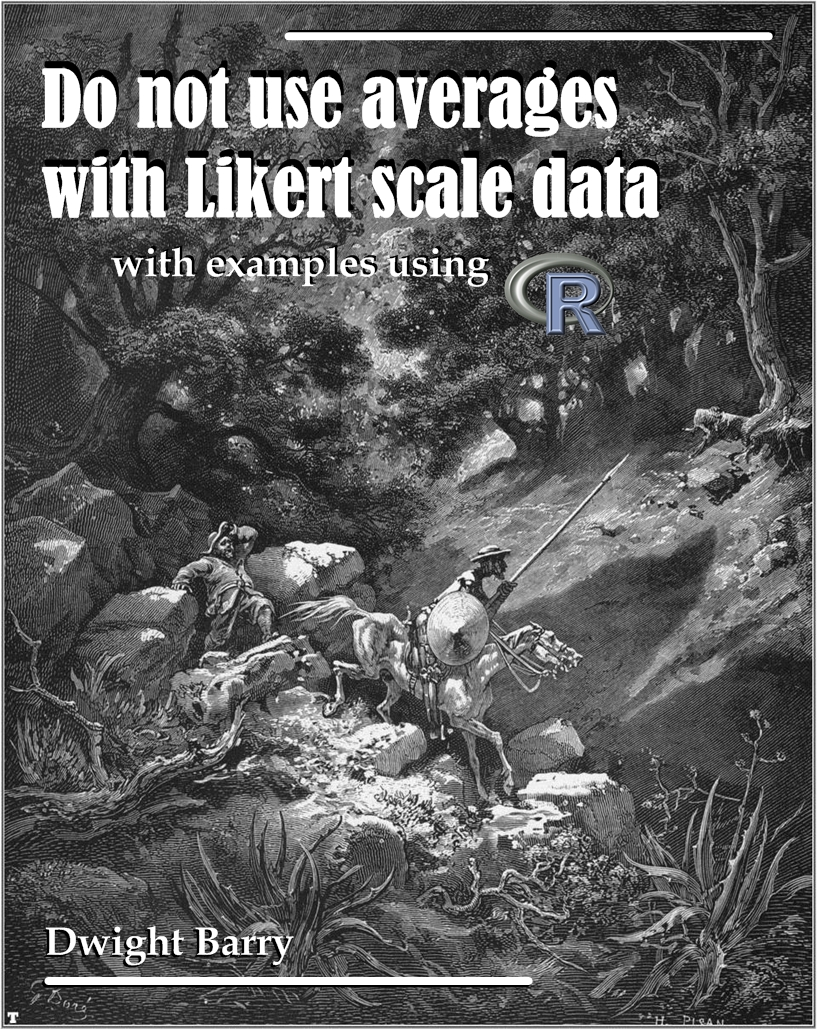
\includegraphics[width=11.35in]{images/likert_cover} \end{center}

This is a short overview of why averages don't work well for evaluating
Likert scale or other ordinal-scale data, and what to do instead, with
examples using R. While the examples are focused on healthcare surveys,
the lessons apply to any use of ordinal scale data.

Note: all of the data in this document is fake, created specifically to
illustrate particular points.

\emph{Contact/Twitter:} \citet{healthstatsdude}

\emph{PDF version:}

\emph{Website:} \url{https://bookdown.org/Rmadillo/likert/}

\emph{Corrections/Pull requests:}
\url{https://github.com/Rmadillo/likert}

\emph{Cover image}: Gustave Doré, 1863. Illustration 12 for Cervantes's
\emph{Don Quixote}.
\href{https://commons.wikimedia.org/w/index.php?curid=677913}{Public
Domain}.


\includegraphics[width=1.22in]{/Users/dbarr1/Documents/R/bookdown/likert/images/cc-by-sa}

\emph{This work is licensed under a
\href{https://creativecommons.org/licenses/by-sa/4.0/}{Creative Commons
Attribution-ShareAlike 4.0 License}.}

\section*{R packgaes}\label{r-packgaes}
\addcontentsline{toc}{section}{R packgaes}

\begin{Shaded}
\begin{Highlighting}[]
\NormalTok{#### Packages ####}
\KeywordTok{library}\NormalTok{(grid)}
\KeywordTok{library}\NormalTok{(nnet)}
\KeywordTok{library}\NormalTok{(coin)}
\KeywordTok{library}\NormalTok{(boot)}
\KeywordTok{library}\NormalTok{(simpleboot)}
\KeywordTok{library}\NormalTok{(knitr)}
\KeywordTok{library}\NormalTok{(ggplot2)}
\KeywordTok{library}\NormalTok{(dplyr)}
\KeywordTok{library}\NormalTok{(AICcmodavg)}
\KeywordTok{library}\NormalTok{(polycor)}
\KeywordTok{library}\NormalTok{(likert)}
\KeywordTok{library}\NormalTok{(MASS)}
\KeywordTok{library}\NormalTok{(ordinal)}
\end{Highlighting}
\end{Shaded}

\section*{Data}\label{data}
\addcontentsline{toc}{section}{Data}

\begin{Shaded}
\begin{Highlighting}[]
\NormalTok{#### Basic example data set ####}
\NormalTok{person =}\StringTok{ }\KeywordTok{c}\NormalTok{(}\StringTok{'A'}\NormalTok{,}\StringTok{'B'}\NormalTok{,}\StringTok{'C'}\NormalTok{,}\StringTok{'D'}\NormalTok{,}\StringTok{'E'}\NormalTok{,}\StringTok{'F'}\NormalTok{)}

\CommentTok{# Original }
\NormalTok{year1 =}\StringTok{ }\KeywordTok{c}\NormalTok{(}\DecValTok{5}\NormalTok{,}\DecValTok{4}\NormalTok{,}\DecValTok{4}\NormalTok{,}\DecValTok{4}\NormalTok{,}\DecValTok{4}\NormalTok{,}\DecValTok{4}\NormalTok{)}
\NormalTok{year2 =}\StringTok{ }\KeywordTok{c}\NormalTok{(}\DecValTok{2}\NormalTok{,}\DecValTok{5}\NormalTok{,}\DecValTok{5}\NormalTok{,}\DecValTok{5}\NormalTok{,}\DecValTok{5}\NormalTok{,}\DecValTok{4}\NormalTok{)}
\NormalTok{year3 =}\StringTok{ }\KeywordTok{c}\NormalTok{(}\DecValTok{3}\NormalTok{,}\DecValTok{5}\NormalTok{,}\DecValTok{5}\NormalTok{,}\DecValTok{5}\NormalTok{,}\DecValTok{5}\NormalTok{,}\DecValTok{3}\NormalTok{)}
\NormalTok{year4 =}\StringTok{ }\KeywordTok{c}\NormalTok{(}\DecValTok{1}\NormalTok{,}\DecValTok{5}\NormalTok{,}\DecValTok{5}\NormalTok{,}\DecValTok{5}\NormalTok{,}\DecValTok{5}\NormalTok{,}\DecValTok{5}\NormalTok{)}

\CommentTok{# A more obvious version}
\CommentTok{# year1 = c(3,3,3,3,3,3)}
\CommentTok{# year2 = c(4,4,4,2,2,2)}
\CommentTok{# year3 = c(5,4,3,3,2,1)}
\CommentTok{# year4 = c(5,5,5,1,1,1)}
 
\NormalTok{ex_1 =}\StringTok{ }\KeywordTok{data.frame}\NormalTok{(person, year1, year2, year3, year4)}
 
\NormalTok{ex_1_long =}\StringTok{ }\NormalTok{reshape2::}\KeywordTok{melt}\NormalTok{(ex_1)}

\NormalTok{#### Larger example data set ####}

\KeywordTok{set.seed}\NormalTok{(}\DecValTok{29}\NormalTok{)}

\NormalTok{md =}\StringTok{ }\KeywordTok{data.frame}\NormalTok{(}\DataTypeTok{Group =} \KeywordTok{as.character}\NormalTok{(}\StringTok{"MD"}\NormalTok{), }
    \DataTypeTok{Response1 =} \KeywordTok{ordered}\NormalTok{(}\KeywordTok{sample}\NormalTok{(}\DecValTok{1}\NormalTok{:}\DecValTok{5}\NormalTok{, }\DecValTok{100}\NormalTok{, }\DataTypeTok{replace=}\NormalTok{T, }\DataTypeTok{prob=}\KeywordTok{c}\NormalTok{(.}\DecValTok{1}\NormalTok{,.}\DecValTok{1}\NormalTok{,.}\DecValTok{1}\NormalTok{,.}\DecValTok{2}\NormalTok{,.}\DecValTok{5}\NormalTok{))), }
    \DataTypeTok{Response2 =} \KeywordTok{ordered}\NormalTok{(}\KeywordTok{sample}\NormalTok{(}\DecValTok{1}\NormalTok{:}\DecValTok{5}\NormalTok{, }\DecValTok{100}\NormalTok{, }\DataTypeTok{replace=}\NormalTok{T, }\DataTypeTok{prob=}\KeywordTok{c}\NormalTok{(.}\DecValTok{1}\NormalTok{,.}\DecValTok{3}\NormalTok{,.}\DecValTok{3}\NormalTok{,.}\DecValTok{25}\NormalTok{,.}\DecValTok{15}\NormalTok{))))}
\NormalTok{rn =}\StringTok{ }\KeywordTok{data.frame}\NormalTok{(}\DataTypeTok{Group =} \KeywordTok{as.character}\NormalTok{(}\StringTok{"RN"}\NormalTok{), }
    \DataTypeTok{Response1 =} \KeywordTok{ordered}\NormalTok{(}\KeywordTok{sample}\NormalTok{(}\DecValTok{1}\NormalTok{:}\DecValTok{5}\NormalTok{, }\DecValTok{100}\NormalTok{, }\DataTypeTok{replace=}\NormalTok{T, }\DataTypeTok{prob=}\KeywordTok{c}\NormalTok{(.}\DecValTok{1}\NormalTok{,.}\DecValTok{1}\NormalTok{,.}\DecValTok{5}\NormalTok{,.}\DecValTok{2}\NormalTok{,.}\DecValTok{1}\NormalTok{))), }
    \DataTypeTok{Response2 =} \KeywordTok{ordered}\NormalTok{(}\KeywordTok{sample}\NormalTok{(}\DecValTok{1}\NormalTok{:}\DecValTok{5}\NormalTok{, }\DecValTok{100}\NormalTok{, }\DataTypeTok{replace=}\NormalTok{T, }\DataTypeTok{prob=}\KeywordTok{c}\NormalTok{(.}\DecValTok{1}\NormalTok{,.}\DecValTok{15}\NormalTok{,.}\DecValTok{45}\NormalTok{,.}\DecValTok{15}\NormalTok{,.}\DecValTok{15}\NormalTok{))))}
 
\NormalTok{both =}\StringTok{ }\KeywordTok{rbind}\NormalTok{(md, rn)}

\CommentTok{# Add some NAs }
\NormalTok{make_NAs =}\StringTok{ }\KeywordTok{sample}\NormalTok{(}\DecValTok{1}\NormalTok{:}\DecValTok{200}\NormalTok{, }\DecValTok{15}\NormalTok{, }\DataTypeTok{replace=}\NormalTok{F)}
\NormalTok{both$Response1[make_NAs] =}\StringTok{ }\OtherTok{NA}
 
\NormalTok{make_NAs2 =}\StringTok{ }\KeywordTok{sample}\NormalTok{(}\DecValTok{1}\NormalTok{:}\DecValTok{200}\NormalTok{, }\DecValTok{15}\NormalTok{, }\DataTypeTok{replace=}\NormalTok{F)}
\NormalTok{both$Response2[make_NAs2] =}\StringTok{ }\OtherTok{NA}

\CommentTok{# Add question names to data}
\KeywordTok{names}\NormalTok{(both) =}\StringTok{ }\KeywordTok{c}\NormalTok{(}\StringTok{"EmployeeType"}\NormalTok{, }
                \StringTok{"My team works well together."}\NormalTok{, }
                \StringTok{"I have the tools I need to do my job."}\NormalTok{)}

\NormalTok{#### Dashboarding pain scores example ####}

\CommentTok{# Create list for random pain scores}
\NormalTok{pain_list =}\StringTok{ }\KeywordTok{list}\NormalTok{()}

\NormalTok{for(i in }\DecValTok{1}\NormalTok{:}\DecValTok{24}\NormalTok{)\{}
  \KeywordTok{set.seed}\NormalTok{(i)}
  \NormalTok{pain_level =}\StringTok{ }\KeywordTok{ordered}\NormalTok{(}\KeywordTok{sample}\NormalTok{(}\KeywordTok{c}\NormalTok{(}\StringTok{"Low"}\NormalTok{, }\StringTok{"Medium"}\NormalTok{, }\StringTok{"High"}\NormalTok{), }\DataTypeTok{size =} \KeywordTok{sample}\NormalTok{(}\DecValTok{10}\NormalTok{:}\DecValTok{30}\NormalTok{),}
    \DataTypeTok{replace =} \NormalTok{T, }\DataTypeTok{prob =} \KeywordTok{c}\NormalTok{(.}\DecValTok{15}\NormalTok{, .}\DecValTok{45}\NormalTok{, .}\DecValTok{40}\NormalTok{)), }\DataTypeTok{levels =} \KeywordTok{c}\NormalTok{(}\StringTok{"Low"}\NormalTok{, }\StringTok{"Medium"}\NormalTok{, }\StringTok{"High"}\NormalTok{))}
  \NormalTok{pain_list[[i]] =}\StringTok{ }\KeywordTok{table}\NormalTok{(pain_level)}
\NormalTok{\}}

\CommentTok{# Unlist into a data frame}
\NormalTok{pain_df =}\StringTok{ }\KeywordTok{data.frame}\NormalTok{(}\KeywordTok{matrix}\NormalTok{(}\KeywordTok{unlist}\NormalTok{(pain_list), }\DataTypeTok{nrow=}\DecValTok{24}\NormalTok{, }\DataTypeTok{byrow=}\NormalTok{T))}
\KeywordTok{colnames}\NormalTok{(pain_df) =}\StringTok{ }\KeywordTok{c}\NormalTok{(}\StringTok{"Low"}\NormalTok{, }\StringTok{"Medium"}\NormalTok{, }\StringTok{"High"}\NormalTok{)}

\CommentTok{# Add some months}
\NormalTok{pain_scores =}\StringTok{ }\KeywordTok{data.frame}\NormalTok{(}\DataTypeTok{Month =} \KeywordTok{seq}\NormalTok{(}\KeywordTok{as.Date}\NormalTok{(}\StringTok{"2014-10-01"}\NormalTok{), }\DataTypeTok{by =} \StringTok{"month"}\NormalTok{, }
  \DataTypeTok{length.out =} \DecValTok{24}\NormalTok{), pain_df)}

\CommentTok{# Melt into long form, I really should learn tidyr}
\NormalTok{pain_scores =}\StringTok{ }\NormalTok{reshape2::}\KeywordTok{melt}\NormalTok{(pain_scores, }\DataTypeTok{id.vars =} \StringTok{"Month"}\NormalTok{, }
  \DataTypeTok{variable.name =} \StringTok{"Pain_Group"}\NormalTok{, }\DataTypeTok{value.name =} \StringTok{"Count"}\NormalTok{)}

\CommentTok{# Summarize to get counts and percentages}
\NormalTok{surgeries_pain =}\StringTok{ }\NormalTok{pain_scores %>%}\StringTok{ }
\StringTok{  }\KeywordTok{group_by}\NormalTok{(Month) %>%}
\StringTok{  }\KeywordTok{mutate}\NormalTok{(}\DataTypeTok{Surgeries =} \KeywordTok{sum}\NormalTok{(Count), }\DataTypeTok{percent =} \NormalTok{(Count /}\StringTok{ }\KeywordTok{sum}\NormalTok{(Count)), }
    \DataTypeTok{cumsum =} \KeywordTok{cumsum}\NormalTok{(percent))}

\NormalTok{#### For use with chi-square and regression models ####}

\CommentTok{# Get rid of NAs}
\NormalTok{both2 =}\StringTok{ }\KeywordTok{na.omit}\NormalTok{(both)}

\CommentTok{# Rename columns to something more R-friendly}
\KeywordTok{names}\NormalTok{(both2) =}\StringTok{ }\KeywordTok{c}\NormalTok{(}\StringTok{"EmployeeType"}\NormalTok{, }\StringTok{"Teamwork"}\NormalTok{, }\StringTok{"Tools"}\NormalTok{)}

\CommentTok{# Reverse the levels so 5 will be at top of mosaic plot}
\NormalTok{both2$Teamwork =}\StringTok{ }\KeywordTok{ordered}\NormalTok{(both2$Teamwork, }\DataTypeTok{levels =} \KeywordTok{c}\NormalTok{(}\StringTok{"5"}\NormalTok{, }\StringTok{"4"}\NormalTok{, }\StringTok{"3"}\NormalTok{, }\StringTok{"2"}\NormalTok{, }\StringTok{"1"}\NormalTok{))}

\CommentTok{# Make a table object}
\NormalTok{both2_tab =}\StringTok{ }\KeywordTok{xtabs}\NormalTok{(~}\StringTok{ }\NormalTok{both2$EmployeeType +}\StringTok{ }\NormalTok{both2$Teamwork)}

\CommentTok{# For multinomial and prop odds models}
\NormalTok{both3 =}\StringTok{ }\NormalTok{both2}

\CommentTok{# Bring axis back to normal}
\NormalTok{both3$Teamwork =}\StringTok{ }\KeywordTok{ordered}\NormalTok{(both3$Teamwork, }\DataTypeTok{levels =} \KeywordTok{c}\NormalTok{(}\StringTok{"1"}\NormalTok{, }\StringTok{"2"}\NormalTok{, }\StringTok{"3"}\NormalTok{, }\StringTok{"4"}\NormalTok{, }\StringTok{"5"}\NormalTok{))}

\CommentTok{# Data frame for proportional odds regression}
\NormalTok{Teamwork_tab_long =}\StringTok{ }\NormalTok{both3[,}\DecValTok{1}\NormalTok{:}\DecValTok{2}\NormalTok{] %>%}
\StringTok{  }\KeywordTok{group_by}\NormalTok{(EmployeeType, Teamwork) %>%}
\StringTok{  }\KeywordTok{summarize}\NormalTok{(}\DataTypeTok{Count =} \KeywordTok{n}\NormalTok{())}

\CommentTok{# Function to turn counts into rows I found laying around the web somewhere}
\NormalTok{countsToCases =}\StringTok{ }\NormalTok{function(x, }\DataTypeTok{countcol =} \StringTok{"Count"}\NormalTok{) \{}
    \CommentTok{# Get the row indices to pull from x}
    \NormalTok{idx =}\StringTok{ }\KeywordTok{rep.int}\NormalTok{(}\KeywordTok{seq_len}\NormalTok{(}\KeywordTok{nrow}\NormalTok{(x)), x[[countcol]])}
    \CommentTok{# Drop count column}
    \NormalTok{x[[countcol]] =}\StringTok{ }\OtherTok{NULL}
    \CommentTok{# Get the rows from x}
    \NormalTok{x[idx, ]}
\NormalTok{\}}

\CommentTok{# Make a data frame for prop odds}
\NormalTok{Teamwork_tab_long$Teamwork_Group =}\StringTok{ }\KeywordTok{as.numeric}\NormalTok{(Teamwork_tab_long$Teamwork) }
\NormalTok{Teamwork_tab_long$Teamwork =}\StringTok{ }\KeywordTok{ordered}\NormalTok{(Teamwork_tab_long$Teamwork) }
\NormalTok{tab_df =}\StringTok{ }\KeywordTok{data.frame}\NormalTok{(}\KeywordTok{countsToCases}\NormalTok{(Teamwork_tab_long, }\DataTypeTok{countcol=}\StringTok{"Count"}\NormalTok{))}
\end{Highlighting}
\end{Shaded}

\chapter{Summary}\label{summary}

\begin{itemize}
\item
  Likert and similar ordinal-level scales have a variety of uses,
  particularly within surveys. They also occur in clinical care, for
  example, in the use of pain scores.
\item
  When evaluated improperly---particularly through the use of
  averages---the results can be strikingly misleading. Obviously,
  misleading results could drive or promote action where none is
  warranted, and vice versa.
\item
  In nearly all cases, not only is it mathematically wrong,
  \textbf{taking the average of a Likert-scale variable will \emph{not}
  provide useful answers} to the questions managers can use to make
  actionable decisions. In essence, the use of averages cannot account
  for the importance of capturing and understanding variability.
  Analysts should strive to avoid their use in any reporting solution or
  analytic product that uses ordinal-scale data.
\item
  Better ways to represent ordinal-value results include histograms of
  the values themselves, the use of well-supported ``top-box''-type
  proportions, and/or bar charts of percentage by score or score
  category (e.g., favorable/neutral/unfavorable).
\item
  ``Statistical significance'' on changes or differences between
  response groups' medians or distribution shift can be assessed through
  non-parametric frequentist tests (e.g., permutation,
  Mann-Whitney-Wilcoxon), Information Theory, or Bayesian analysis.
  \emph{t}-tests should never be used on Likert scales because ordinal
  data does not meet the assumptions of a \emph{t}-test (and when using
  frequentist tools, one must \emph{also} account for multiple testing
  to reduce the chance of false positives).
\item
  A good way to remember not to use means on Likert scale data is to
  think: The average of \emph{Agree} and \emph{Strongly Agree} is
  \textbf{not} \emph{Agree-And-A-Half}.
\end{itemize}

\chapter{\texorpdfstring{\emph{Why not?} A simple
example}{Why not? A simple example}}\label{why-not-a-simple-example}

Take a simple example where a group of 6 people people take the same
survey for 4 years, and the mean results for an important question, such
as ``my team works well together'', are as follows:

\begin{tabular}{l|r}
\hline
Year & Mean\\
\hline
Year 1 & 4.17\\
\hline
Year 2 & 4.33\\
\hline
Year 3 & 4.33\\
\hline
Year 4 & 4.33\\
\hline
\end{tabular}

From these values, one might conclude that there is an improvement from
year 1 to year 2, and no change year-over-year after year 2.

The values that created the above results are as follows:

\begin{tabular}{l|r|r|r|r}
\hline
Individual & Year 1 & Year 2 & Year 3 & Year 4\\
\hline
A & 5 & 2 & 3 & 1\\
\hline
B & 4 & 5 & 5 & 5\\
\hline
C & 4 & 5 & 5 & 5\\
\hline
D & 4 & 5 & 5 & 5\\
\hline
E & 4 & 5 & 5 & 5\\
\hline
F & 4 & 4 & 3 & 5\\
\hline
\end{tabular}

You might already see how management decisions would be made differently
based on whether one had just the means or had the complete data.

However, in the latter case, you risk reducing or eliminating anonymity,
which is essential to get respondents to answer truthfully (not to
mention being unethical). Further, poring over tables of answers for
many people for long surveys makes that approach practically infeasible.

Visualizing the results in ways that capture a more complete story
provides an answer to both issues, as well as providing decision-makers
with truly actionable information.

\chapter{\texorpdfstring{\emph{Always}
visualize}{Always visualize}}\label{always-visualize}

\section{Histograms}\label{histograms}

Histograms of the actual score values are the best way to visualize
Likert data---they have two real axes, showing counts by score value or
category, so you can parse the visual and understand the results very
quickly. Using the same data as above, you can instantly see that the
``improvement'' in year 2 was perhaps not an improvement after all:
while most respondents appear to be satisfied above what they thought in
year 1, one respondent may be at risk of leaving.

\emph{Histogram of simple example Likert scale data.}

\begin{Shaded}
\begin{Highlighting}[]
\CommentTok{# Figure 1}
\KeywordTok{ggplot}\NormalTok{(ex_1_long, }\KeywordTok{aes}\NormalTok{(value)) +}
\StringTok{    }\KeywordTok{geom_histogram}\NormalTok{(}\DataTypeTok{binwidth=}\DecValTok{1}\NormalTok{) +}
\StringTok{    }\KeywordTok{facet_wrap}\NormalTok{(~variable, }\DataTypeTok{ncol=}\DecValTok{1}\NormalTok{) +}
\StringTok{    }\KeywordTok{xlab}\NormalTok{(}\StringTok{"Likert Scale Value"}\NormalTok{) +}
\StringTok{    }\KeywordTok{theme_bw}\NormalTok{()}
\end{Highlighting}
\end{Shaded}

\begin{center}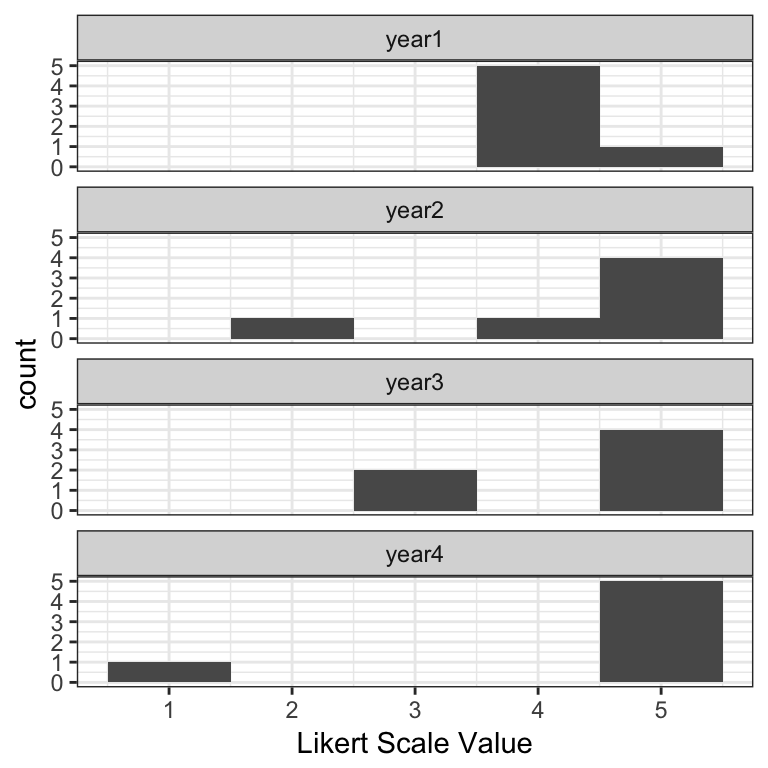
\includegraphics{likert_files/figure-latex/histos-1} \end{center}

\section{Likert charts}\label{likert-charts}

The main disadvantage of histograms is space; Likert charts---which are
in essence just stacked bar charts---are far more compact. The
disadvantage is that it takes slightly longer for a user to parse them,
but when faced with lots of questions or groupings, they tend to be a
better option.

There are two kinds of Likert charts---those that use a center line for
a point of reference, and those that do not, in which case they are
simply percentage bar charts for individual questions or are mosaic
plots when comparing groupings. In the graphs below, each score value
has its own color, and each score category---e.g., unfavorable is 1-2,
neutral is 3, and favorable is 4-5 on a 5-point scale---is summarized by
a percentage value at the left, middle/interior, and right sides of the
bar, respectively.

The \texttt{likert} package provides some out-of-the-box plots for this
type of data, though you must convert the numeric values to factors for
it to work.

\emph{Centered Likert chart.}

\begin{Shaded}
\begin{Highlighting}[]
\CommentTok{# Covert values to factors}
\NormalTok{ex_1[}\DecValTok{2}\NormalTok{:}\DecValTok{5}\NormalTok{] =}\StringTok{ }\KeywordTok{lapply}\NormalTok{(ex_1[}\DecValTok{2}\NormalTok{:}\DecValTok{5}\NormalTok{], factor, }\DataTypeTok{levels =} \DecValTok{1}\NormalTok{:}\DecValTok{5}\NormalTok{)}

\CommentTok{# Create a likert object}
\NormalTok{ex_1_likert =}\StringTok{ }\KeywordTok{likert}\NormalTok{(ex_1[}\DecValTok{2}\NormalTok{:}\DecValTok{5}\NormalTok{])}

\CommentTok{# Figure 2}
\KeywordTok{plot}\NormalTok{(ex_1_likert, }\DataTypeTok{ordered =} \OtherTok{FALSE}\NormalTok{, }\DataTypeTok{group.order =} \KeywordTok{names}\NormalTok{(ex_1[}\DecValTok{2}\NormalTok{:}\DecValTok{5}\NormalTok{]))}
\end{Highlighting}
\end{Shaded}

\begin{center}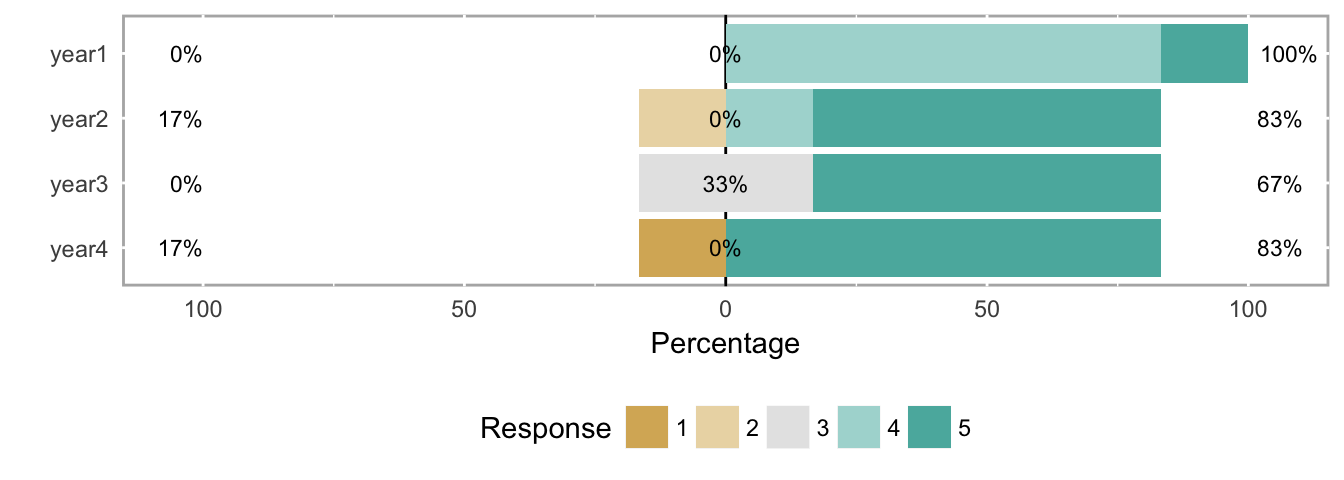
\includegraphics{likert_files/figure-latex/ex_1_likert-1} \end{center}

\emph{Uncentered Likert chart (aka percent bar chart).}

\begin{Shaded}
\begin{Highlighting}[]
\CommentTok{# Figure 3}
\KeywordTok{plot}\NormalTok{(ex_1_likert, }\DataTypeTok{ordered =} \OtherTok{FALSE}\NormalTok{, }\DataTypeTok{centered =} \OtherTok{FALSE}\NormalTok{, }\DataTypeTok{group.order=}\KeywordTok{names}\NormalTok{(ex_1[}\DecValTok{2}\NormalTok{:}\DecValTok{5}\NormalTok{]))}
\end{Highlighting}
\end{Shaded}

\begin{center}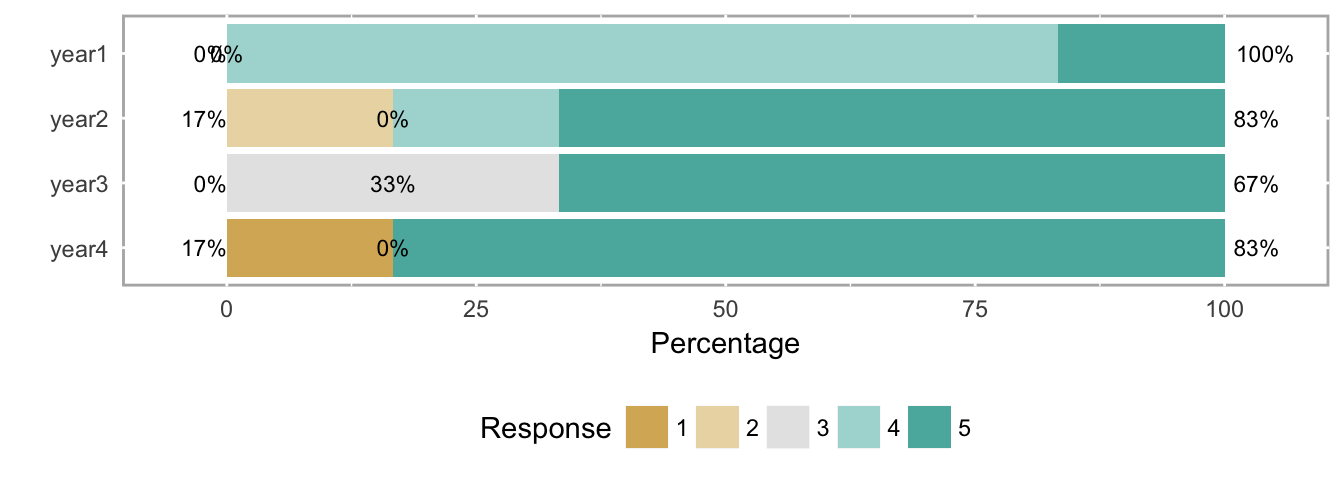
\includegraphics{likert_files/figure-latex/ex_1_likert_percent-1} \end{center}

Neither Likert chart type is as clear as the histogram at making the
results immediately understandable, but again, histograms take more
space, and busy decision makers often need to see the forest (all the
questions) at the expense of some trees (each question). In this case,
analysts might use the histograms to explore potentially important
results themselves, and then use Likert charts in a report with some
strategically-placed text highlighting important patterns they found
with the histograms.

\section{Other ordinal-scale
visualizations}\label{other-ordinal-scale-visualizations}

We'll use a larger data set in this section to illustrate other
visualizations of ordinal data.

\begin{Shaded}
\begin{Highlighting}[]
\CommentTok{# Create likert object for example data set 2}
\NormalTok{ex_2_likert =}\StringTok{ }\KeywordTok{likert}\NormalTok{(both[}\DecValTok{2}\NormalTok{:}\DecValTok{3}\NormalTok{])}
\end{Highlighting}
\end{Shaded}

\subsection{Heatmap}\label{heatmap}

Figure 4 shows a heatmap of the response frequency for two different
questions (e.g., as within a single year's survey). While the use of
means and SDs is inappropriate, this particular example directly
illustrates why those values don't capture the response patterns in the
data.

\emph{Heatmap of the response frequency for two different questions.}

\begin{Shaded}
\begin{Highlighting}[]
\CommentTok{# Figure 4}
\KeywordTok{plot}\NormalTok{(ex_2_likert, }\DataTypeTok{type =} \StringTok{"heat"}\NormalTok{)}
\end{Highlighting}
\end{Shaded}

\begin{center}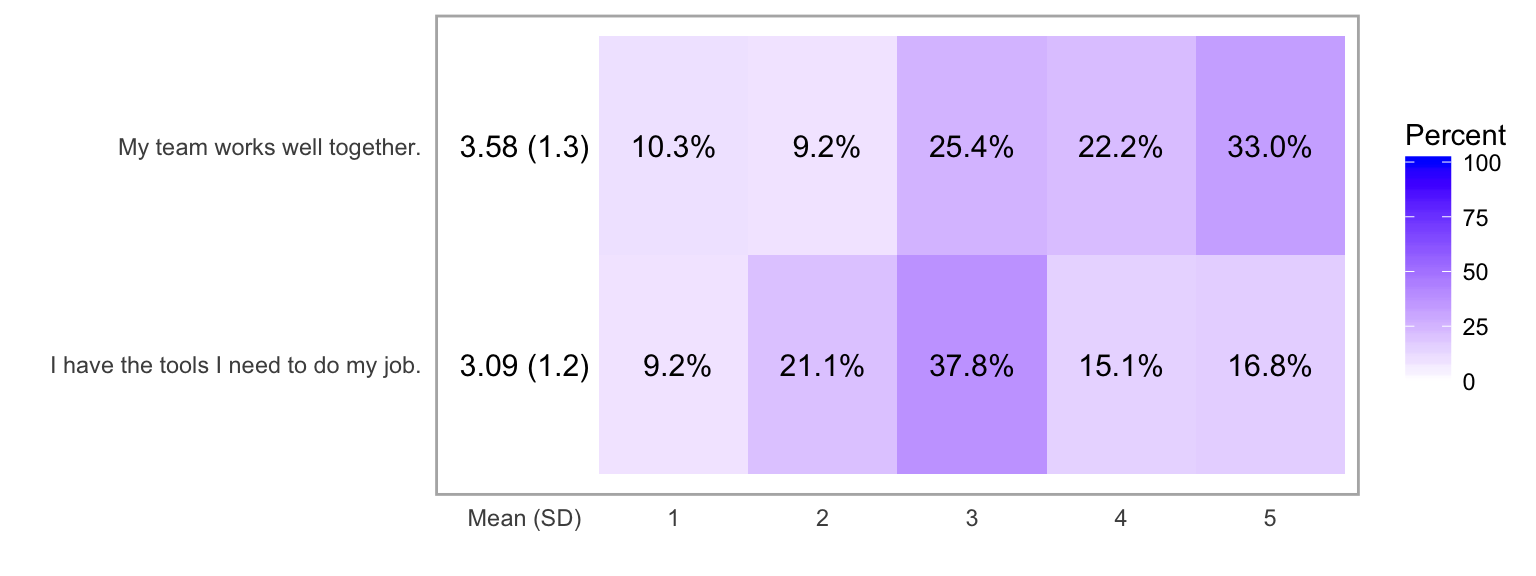
\includegraphics{likert_files/figure-latex/likert_viz3-1} \end{center}

\subsection{Likert chart with response count
histograms}\label{likert-chart-with-response-count-histograms}

The same data as seen in the heatmap above is more clearly shown with a
Likert chart. Another option available with \texttt{likert} objects is
to include count histogram to show number of responses and non-answers
for each question.

\emph{Likert chart of the response frequency for two different
questions.}

\begin{Shaded}
\begin{Highlighting}[]
\CommentTok{# Figure 5}
\KeywordTok{plot}\NormalTok{(ex_2_likert, }\DataTypeTok{include.histogram =} \OtherTok{TRUE}\NormalTok{)}
\end{Highlighting}
\end{Shaded}

\begin{center}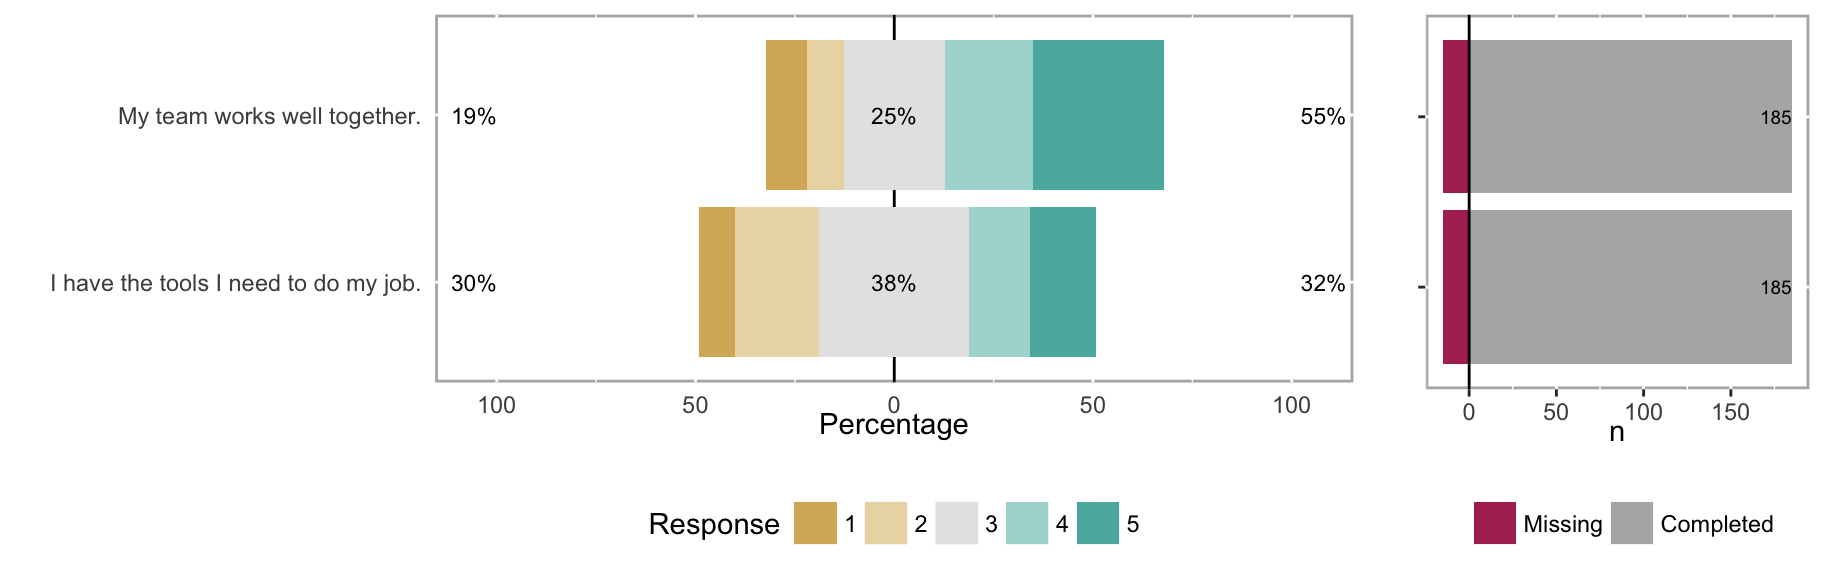
\includegraphics{likert_files/figure-latex/likert_viz1-1} \end{center}

\subsection{Likert chart with
subgroups}\label{likert-chart-with-subgroups}

Subgroups can sometimes reveal patterns not seen in aggregate data. For
example, compare the overall results for ``My team works well together''
in Figure 5 with the responses when broken out by the subgroups of MDs
and RNs in Figure 6.

\emph{Likert chart of the response frequency for two different
questions, grouped by MDs and RNs.}

\begin{Shaded}
\begin{Highlighting}[]
\CommentTok{# Create likert object with groupings included}
\NormalTok{both_likert_2 =}\StringTok{ }\KeywordTok{likert}\NormalTok{(both[, }\KeywordTok{c}\NormalTok{(}\DecValTok{2}\NormalTok{:}\DecValTok{3}\NormalTok{), }\DataTypeTok{drop =} \OtherTok{FALSE}\NormalTok{], }\DataTypeTok{grouping =} \NormalTok{both$EmployeeType)}

\CommentTok{# Figure 6}
\KeywordTok{plot}\NormalTok{(both_likert_2, }\DataTypeTok{include.histogram =} \OtherTok{TRUE}\NormalTok{)}
\end{Highlighting}
\end{Shaded}

\begin{center}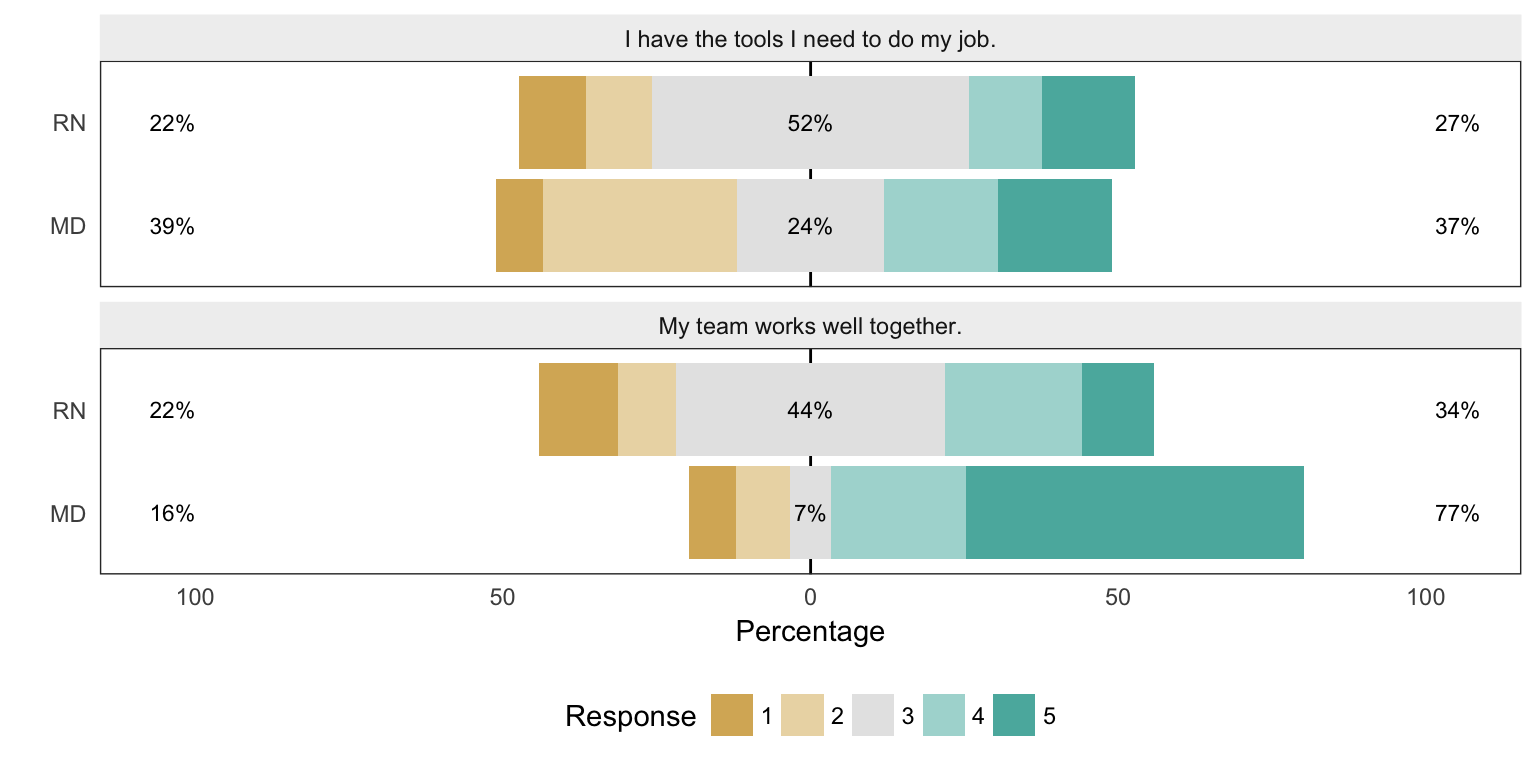
\includegraphics{likert_files/figure-latex/likert_viz4-1} \end{center}

\subsection{Density histograms}\label{density-histograms}

While using a density plot on ordinal data is also statistically
inappropriate, it can be a useful tool for an analyst. Bar histograms
are difficult to overlay subgroups or different years for a direct
comparsion, so must be separated into facets instead, as was seen in
Figure 1. Density plots are easier to overlay to show these comparisons,
so while not appropriate for a report or dashboard, they can be really
useful tools for an analyst during the exploration phase.

\emph{Density histograms of the response frequency for two different
questions, with a grouping variable (MDs and RNs).}

\begin{Shaded}
\begin{Highlighting}[]
\CommentTok{# Figure 7}
\KeywordTok{plot}\NormalTok{(both_likert_2, }\DataTypeTok{type =} \StringTok{"density"}\NormalTok{)}
\end{Highlighting}
\end{Shaded}

\begin{center}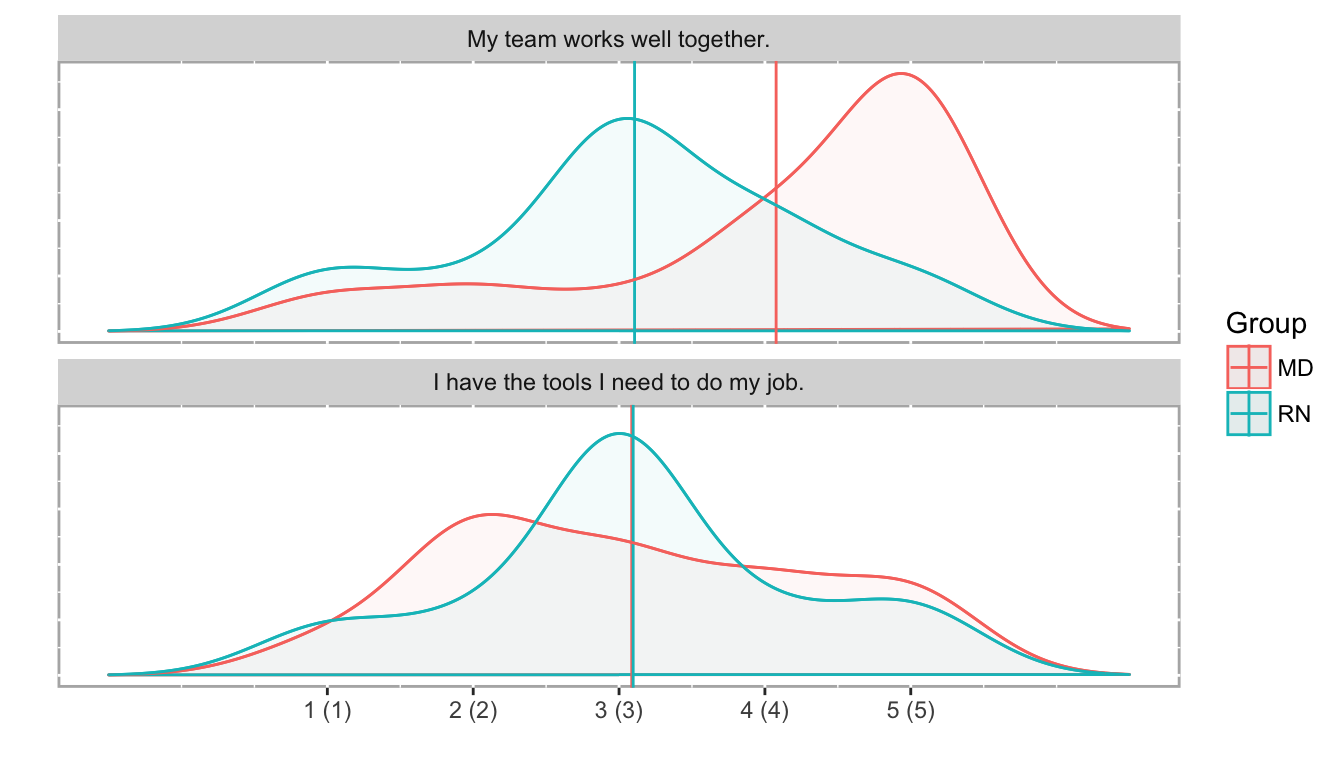
\includegraphics{likert_files/figure-latex/likert_viz5-1} \end{center}

\subsection{Scatterplots \& ordinal
correlation}\label{scatterplots-ordinal-correlation}

Although traditionally many analysts used non-parametric correlation
like Spearman's or Kendall's,
\href{https://en.wikipedia.org/wiki/Polychoric_correlation}{polychoric
correlation} is the proper tool to assess similarities between Likert
scale results. (Polyserial correlation is used when one variable is
numeric and the other is ordinal.)

\begin{Shaded}
\begin{Highlighting}[]
\NormalTok{poly_c_both =}\StringTok{ }\KeywordTok{polychor}\NormalTok{(both[,}\DecValTok{2}\NormalTok{], both[,}\DecValTok{3}\NormalTok{])}
\end{Highlighting}
\end{Shaded}

The polychoric correlation coefficient between ``My team works well
together'' and ``I have the tools I need to do my job'' is 0.0579. As
expected, that suggests that there is no relationship between the
responses to these two questions. It's fairly easy to see this lack of
relationship in a scatterplot, with the points jittered to give a sense
of response density.

\emph{Scatterplot of ordinal comparisons (jittered to show point
density) between the questions `My team works well together' and `I have
the tools I need to do my job'.}

\begin{Shaded}
\begin{Highlighting}[]
\CommentTok{# Figure 8}
\KeywordTok{ggplot}\NormalTok{(both, }\KeywordTok{aes}\NormalTok{(both[,}\DecValTok{2}\NormalTok{], both[,}\DecValTok{3}\NormalTok{], }\DataTypeTok{group=}\NormalTok{EmployeeType, }\DataTypeTok{color=}\NormalTok{EmployeeType)) +}
\StringTok{  }\KeywordTok{geom_jitter}\NormalTok{(}\DataTypeTok{na.rm=}\OtherTok{TRUE}\NormalTok{, }\DataTypeTok{width =} \FloatTok{0.15}\NormalTok{, }\DataTypeTok{height =} \FloatTok{0.15}\NormalTok{, }\DataTypeTok{alpha=}\FloatTok{0.6}\NormalTok{, }\DataTypeTok{size=}\DecValTok{3}\NormalTok{) +}
\StringTok{  }\KeywordTok{xlab}\NormalTok{(}\StringTok{"My team works well together"}\NormalTok{) +}\StringTok{ }
\StringTok{  }\KeywordTok{ylab}\NormalTok{(}\StringTok{"I have the tools I need to do my job"}\NormalTok{) +}
\StringTok{  }\KeywordTok{coord_equal}\NormalTok{()}
\end{Highlighting}
\end{Shaded}

\begin{center}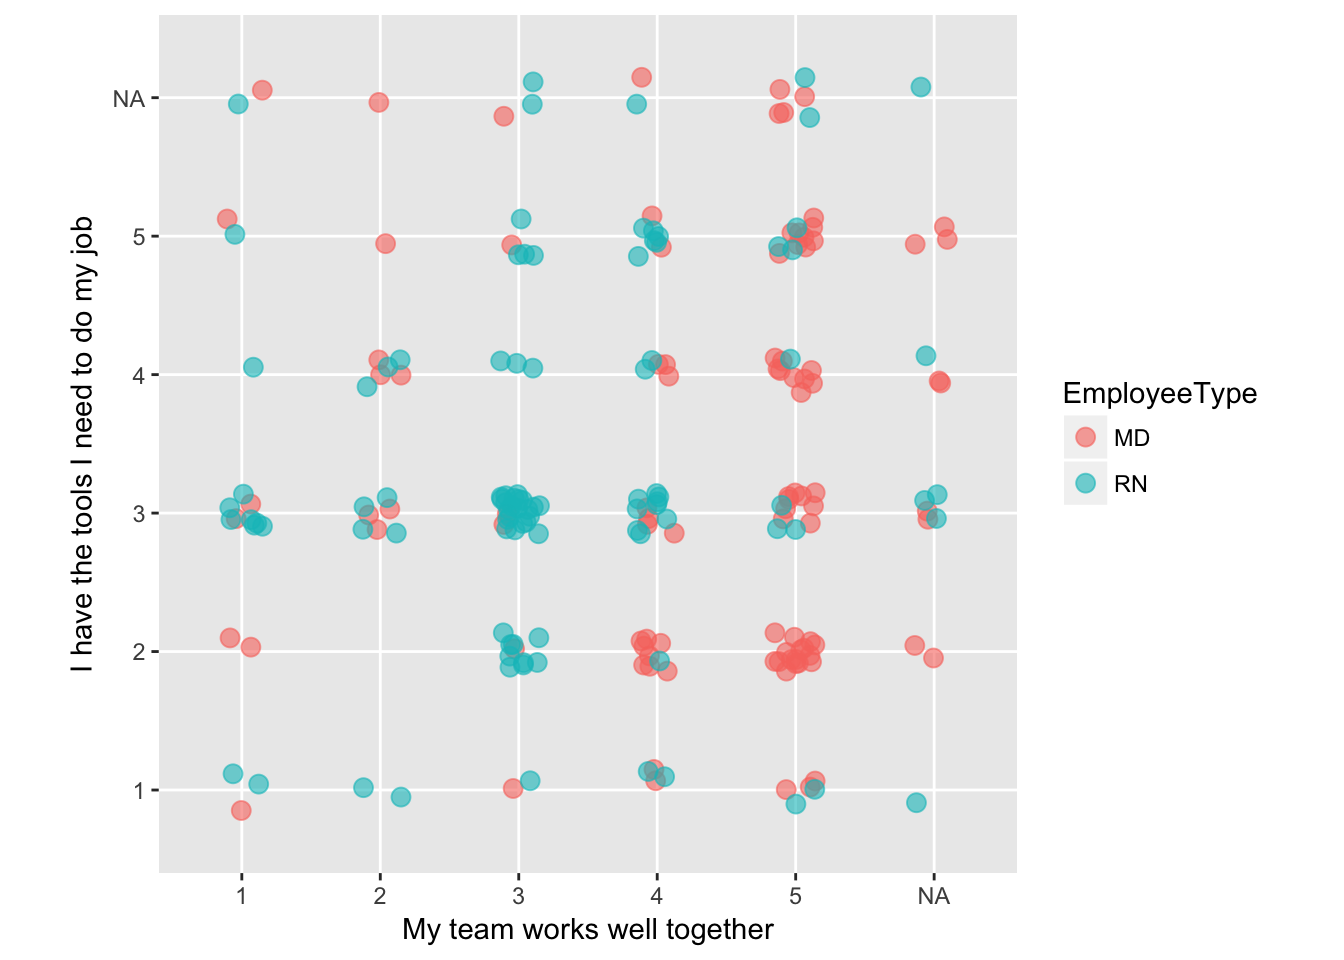
\includegraphics{likert_files/figure-latex/polyc_plot-1} \end{center}

\subsection{Monitoring ordinal data}\label{monitoring-ordinal-data}

In some cases, you may want to monitor data that uses an ordinal scale.
If your metric is a ``top box'' type of score, a simple line chart can
show that data over time; if it's monitoring a stable process,
statistical process control methods can be used as well.

If you want to monitor a more complete view of the data, a stacked
percentage bar chart shows you trends across the time series.

Pain scores are a common outcome measure in surgeries, which are usually
recorded on an intensity scale of 1-10, with 10 being the highest pain
imaginable. Many researchers and quality improvement analysts collapse
those values into Low (1-3), Medium (4-7), and High (8-10) categories,
as the meaning of the exact values varies from patient to patient as
well as between clinicians.

In this example (Figure 9), the maximum pain score for each patient in
the 24 hours following a surgery are recorded, and assigned to a pain
category. The total number of patients with maximum pain scores in each
pain category are summed each month.

\emph{Monitoring maximum pain scores with a stacked percentage bar
chart. Total surgeries performed that month occur just below each bar.}

\begin{Shaded}
\begin{Highlighting}[]
\CommentTok{# Figure 9}
\KeywordTok{ggplot}\NormalTok{(surgeries_pain, }\KeywordTok{aes}\NormalTok{(}\DataTypeTok{x =} \NormalTok{Month, }\DataTypeTok{y =} \NormalTok{Count, }\DataTypeTok{fill =} \NormalTok{Pain_Group)) +}
\StringTok{  }\KeywordTok{geom_bar}\NormalTok{(}\DataTypeTok{position =} \StringTok{"fill"}\NormalTok{, }\DataTypeTok{stat =} \StringTok{"identity"}\NormalTok{) +}
\StringTok{  }\KeywordTok{scale_y_continuous}\NormalTok{(}\DataTypeTok{labels =} \NormalTok{scales::percent) +}
\StringTok{  }\KeywordTok{scale_fill_brewer}\NormalTok{(}\DataTypeTok{name =} \StringTok{"Pain Groups:"}\NormalTok{, }\DataTypeTok{type =} \StringTok{"div"}\NormalTok{, }\DataTypeTok{palette =} \StringTok{"Spectral"}\NormalTok{, }\DataTypeTok{direction =} \NormalTok{-}\DecValTok{1}\NormalTok{) +}
\StringTok{  }\KeywordTok{geom_text}\NormalTok{(}\KeywordTok{aes}\NormalTok{(}\DataTypeTok{y =} \NormalTok{-}\FloatTok{0.02}\NormalTok{, }\DataTypeTok{label =} \NormalTok{Surgeries), }\DataTypeTok{size =} \DecValTok{2}\NormalTok{, }\DataTypeTok{color =} \StringTok{"gray40"}\NormalTok{) +}
\StringTok{  }\KeywordTok{ylab}\NormalTok{(}\StringTok{"Proportion"}\NormalTok{) +}\StringTok{ }
\StringTok{  }\KeywordTok{theme_bw}\NormalTok{() +}
\StringTok{  }\KeywordTok{theme}\NormalTok{(}\DataTypeTok{legend.position =} \StringTok{"top"}\NormalTok{)}
\end{Highlighting}
\end{Shaded}

\begin{center}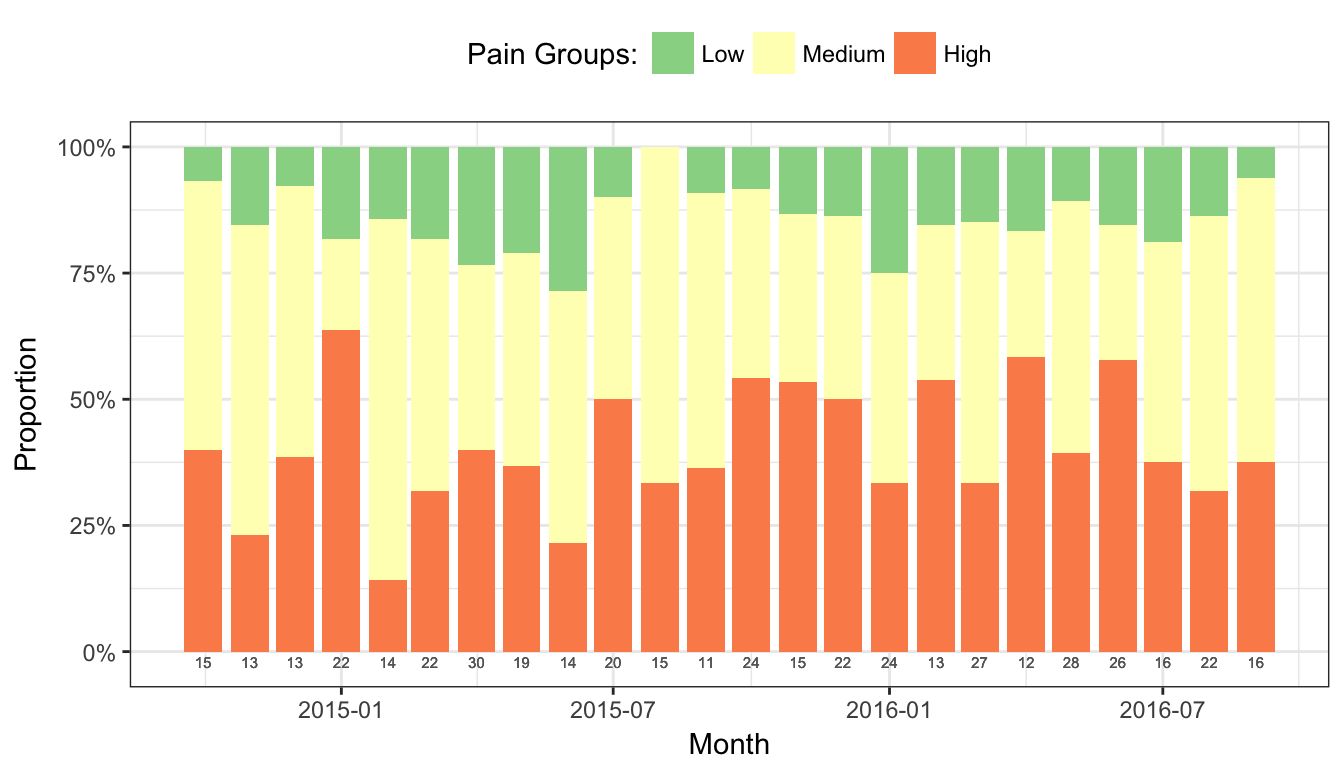
\includegraphics{likert_files/figure-latex/monitoring-1} \end{center}

\chapter{\texorpdfstring{\emph{Neutral} scores
matter}{Neutral scores matter}}\label{neutral-scores-matter}

You might have noticed in some surveys that there is often no
``neutral'' or ``undecided'' category included in the middle of the
scale, e.g., what's usually a 3 on a 5-point Likert scale. Sometimes it
is placed at the end of the scale, and sometimes it is eliminated
entirely. The reason for this is that those terms can sometimes be
interpreted in a variety of ways; for example, with a question such as
``My pay is fair compared with other companies'', a \emph{Neutral}
response could indicate ``I'm neutral on this'', ``yes, I guess so'',
``I don't know'', ``it's neither fair nor unfair'', ``I don't want to
answer'', ``I'm not sure what `fair' means'', and any number of ideas
that don't necessarily indicate a true neutral opinion.

When a question has a response option where this type of ambiguity
exists, a mean value will tend toward the that option because of this
bias, unless of course the mean is already at that value. However, when
\emph{Neutral} is marked as 3, and when valid responses tend towards 4s
and 5s, these ambiguous responses will drag down the average (and vice
versa for responses heavy with 1s and 2s). Of course, you shouldn't use
means anyway, as we've seen above, but many reports do---so
understanding this effect is important toward interpreting the results
in a useful way.

Use of a median is somewhat resistant to this problem, though you still
won't know whether the middle values are valid responses or accidents of
interpretation.

When you see an ``undecided'' or ``N/A'' response placed at the end of
the scale or missing entirely, it is usually (but not always!) a sign
that the survey creator understands this problem.

Sometimes, of course, \emph{Neutral} can be a completely reasonable and
unambiguous response to a question. Context matters; while it's easiest
for survey creators and scanning software to use the same scale for
large numbers of questions, it is important that the analyst understand
the extent to which \emph{Neutral} and similar types of responses are a
valid part of the measurement scale for each question.

\begin{center}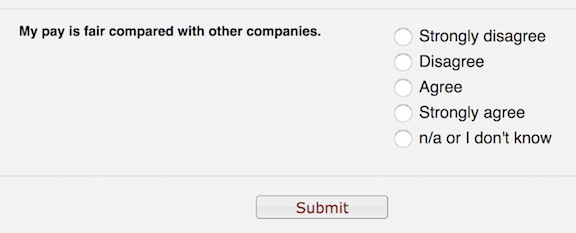
\includegraphics[width=8in]{images/no_neutral} \end{center}

\chapter{How many respondents are
enough?}\label{how-many-respondents-are-enough}

It's common to think: ``We surveyed everyone in this department,
therefore the results we see must be correct.'' However, how people
responded to surveys depends on many factors---such as mood the date the
survey is taken, recent events in life and in work, changes in
organizational structure, and any number of other factors---and many
internal surveys are given only once a year. Thus, survey results are
really a \emph{sample} of attitudes and opinions, subject to random
events and natural fluctuations.

Typical practice at some companies is to expose summary results for
groups with six or more people. While this helps preserve some
anonymity, it does not include enough responses to ensure the overall
response is stable. Comparisons over time or across groups that are not
based on stable results can lead to conclusions about differences that
may or may not reflect reality.

In this context, \emph{stable} means that the data accurately represent
true changes (or lack of change) in the question at hand. It's basically
impossible to distinguish natural variation from real change when you
have small numbers of respondents. As a result, the National Center for
Health Statistics, for example, does not publish results with less than
20 distinct cases or responses.

The relative standard error (RSE) is the metric used to evaluate whether
you have enough values for the results to be stable. The standard error
is an estimate of the likely difference between the results and the true
value (which in surveys, even of complete populations, can't be known
exactly due to the reasons mentioned above). The \emph{relative}
standard error is the standard error expressed as a percent of the
measure or number of responses, which is a constant function:
\(\frac{1}{\sqrt{responses}} * 100\). This function can be seen in the
graph on the next page.

Generally, you want RSE values less than 20-25\% to have some confidence
that your results are stable.\\
The RSE-response count function is shown in Figure 10. The RSE
associated with the use of six responses is marked with dark red, and
the response count associated with an RSE of 25\% is marked with dark
blue.

\begin{Shaded}
\begin{Highlighting}[]
\NormalTok{x =}\StringTok{ }\KeywordTok{seq}\NormalTok{(}\DecValTok{1}\NormalTok{:}\DecValTok{50}\NormalTok{)}
\NormalTok{rse =}\StringTok{ }\KeywordTok{data.frame}\NormalTok{(}\DataTypeTok{x =} \NormalTok{x, }\DataTypeTok{y =} \NormalTok{(}\DecValTok{1} \NormalTok{/}\StringTok{ }\KeywordTok{sqrt}\NormalTok{(x)) *}\StringTok{ }\DecValTok{100}\NormalTok{)}

\CommentTok{# Figure 10}
\KeywordTok{ggplot}\NormalTok{(rse, }\KeywordTok{aes}\NormalTok{(}\DataTypeTok{x =} \NormalTok{x, }\DataTypeTok{y =} \NormalTok{y)) +}
\StringTok{  }\KeywordTok{geom_line}\NormalTok{() +}
\StringTok{  }\KeywordTok{geom_segment}\NormalTok{(}\KeywordTok{aes}\NormalTok{(}\DataTypeTok{x=}\DecValTok{6}\NormalTok{, }\DataTypeTok{y=}\DecValTok{0}\NormalTok{, }\DataTypeTok{xend=}\DecValTok{6}\NormalTok{, }\DataTypeTok{yend=}\DecValTok{41}\NormalTok{), }\DataTypeTok{color=}\StringTok{"darkred"}\NormalTok{, }\DataTypeTok{arrow =} \KeywordTok{arrow}\NormalTok{(}\DataTypeTok{length =} \KeywordTok{unit}\NormalTok{(}\FloatTok{0.25}\NormalTok{, }\StringTok{"cm"}\NormalTok{))) +}
\StringTok{  }\KeywordTok{geom_segment}\NormalTok{(}\KeywordTok{aes}\NormalTok{(}\DataTypeTok{x=}\DecValTok{6}\NormalTok{, }\DataTypeTok{y=}\DecValTok{41}\NormalTok{, }\DataTypeTok{xend=}\DecValTok{0}\NormalTok{, }\DataTypeTok{yend=}\DecValTok{41}\NormalTok{), }\DataTypeTok{color=}\StringTok{"darkred"}\NormalTok{, }\DataTypeTok{arrow =} \KeywordTok{arrow}\NormalTok{(}\DataTypeTok{length =} \KeywordTok{unit}\NormalTok{(}\FloatTok{0.25}\NormalTok{, }\StringTok{"cm"}\NormalTok{))) +}
\StringTok{  }\KeywordTok{geom_label}\NormalTok{(}\KeywordTok{aes}\NormalTok{(}\DataTypeTok{x=}\DecValTok{6}\NormalTok{, }\DataTypeTok{y=}\NormalTok{-}\DecValTok{5}\NormalTok{), }\DataTypeTok{label =} \StringTok{"6"}\NormalTok{) +}
\StringTok{  }\KeywordTok{geom_label}\NormalTok{(}\KeywordTok{aes}\NormalTok{(}\DataTypeTok{x=}\NormalTok{-}\FloatTok{1.75}\NormalTok{, }\DataTypeTok{y=}\DecValTok{41}\NormalTok{), }\DataTypeTok{label =} \StringTok{"41"}\NormalTok{) +}
\StringTok{  }\KeywordTok{geom_segment}\NormalTok{(}\KeywordTok{aes}\NormalTok{(}\DataTypeTok{x=}\DecValTok{16}\NormalTok{, }\DataTypeTok{y=}\DecValTok{25}\NormalTok{, }\DataTypeTok{xend=}\DecValTok{16}\NormalTok{, }\DataTypeTok{yend=}\DecValTok{0}\NormalTok{), }\DataTypeTok{color=}\StringTok{"darkblue"}\NormalTok{, }\DataTypeTok{arrow =} \KeywordTok{arrow}\NormalTok{(}\DataTypeTok{length =} \KeywordTok{unit}\NormalTok{(}\FloatTok{0.25}\NormalTok{, }\StringTok{"cm"}\NormalTok{))) +}
\StringTok{  }\KeywordTok{geom_segment}\NormalTok{(}\KeywordTok{aes}\NormalTok{(}\DataTypeTok{x=}\DecValTok{0}\NormalTok{, }\DataTypeTok{y=}\DecValTok{25}\NormalTok{, }\DataTypeTok{xend=}\DecValTok{16}\NormalTok{, }\DataTypeTok{yend=}\DecValTok{25}\NormalTok{), }\DataTypeTok{color=}\StringTok{"darkblue"}\NormalTok{, }\DataTypeTok{arrow =} \KeywordTok{arrow}\NormalTok{(}\DataTypeTok{length =} \KeywordTok{unit}\NormalTok{(}\FloatTok{0.25}\NormalTok{, }\StringTok{"cm"}\NormalTok{))) +}
\StringTok{  }\KeywordTok{geom_label}\NormalTok{(}\KeywordTok{aes}\NormalTok{(}\DataTypeTok{x=}\DecValTok{16}\NormalTok{, }\DataTypeTok{y=}\NormalTok{-}\DecValTok{5}\NormalTok{), }\DataTypeTok{label =} \StringTok{"16"}\NormalTok{) +}
\StringTok{  }\KeywordTok{geom_label}\NormalTok{(}\KeywordTok{aes}\NormalTok{(}\DataTypeTok{x=}\NormalTok{-}\FloatTok{1.75}\NormalTok{, }\DataTypeTok{y=}\DecValTok{25}\NormalTok{), }\DataTypeTok{label =} \StringTok{"25"}\NormalTok{) +}
\StringTok{  }\KeywordTok{xlab}\NormalTok{(}\StringTok{"Number of responses"}\NormalTok{) +}
\StringTok{  }\KeywordTok{ylab}\NormalTok{(}\StringTok{"Relative Standard Error"}\NormalTok{)}
\end{Highlighting}
\end{Shaded}

\begin{center}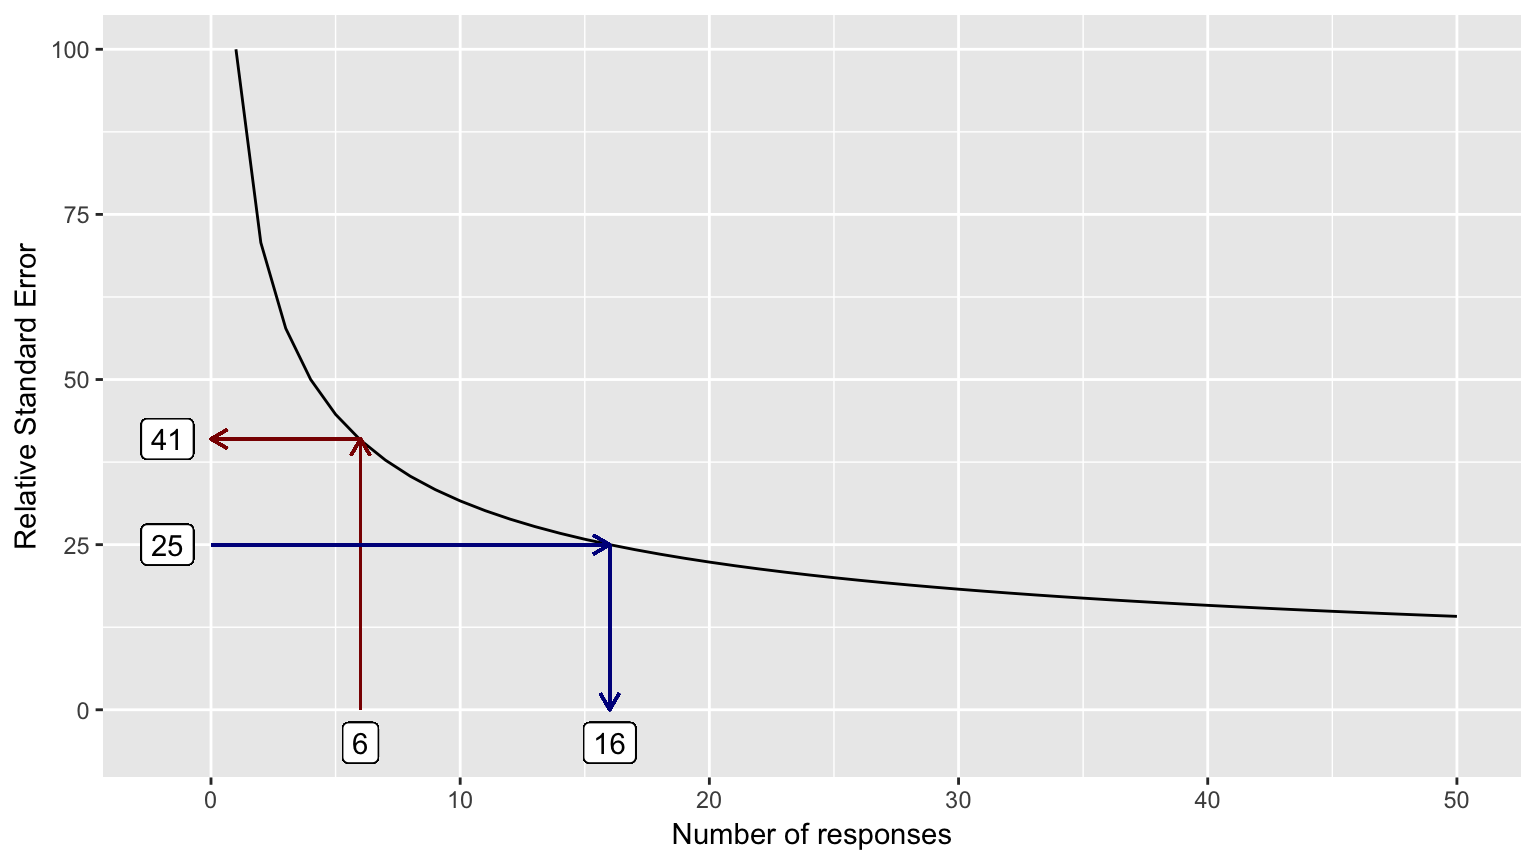
\includegraphics{likert_files/figure-latex/rse-1} \end{center}

\chapter{\texorpdfstring{Is there a \emph{significant}
difference?}{Is there a significant difference?}}\label{is-there-a-significant-difference}

Many decision-makers want to know if a result is ``significantly
different'' from, say, the same response from a previous time period, or
between a couple of subgroups in the same response, typically asking for
identification of questions in which \emph{p} \textless{} 0.05 using a
\emph{t}-test. Unfortunately, this is mostly useless, for two reasons.

First, acting as if Likert or other ordinal scales are continuous level
data leads to many problems of interpretation (see the \emph{Appendix}
for a summary table of measurement scales and appropriate statistics).
There has been controversy over this distinction for many decades;
however, a great way to understand the conceptual problem is to realize
that the mean of \emph{Agree} and \emph{Strongly Agree} is \textbf{not}
\emph{Agree-And-A-Half}---it just makes no sense.

A subsequent argument might be that, no, it's not conceptually accurate,
but it provides a sense for directional changes. However, such results
still run into problems of interpretation: if you go from 4.17 to 4.33,
have you gone from \emph{Agree.17} to \emph{Agree.33}? What does such an
``improvement'' mean, in practical terms? All you can accurately say is
that both values are most consistent with an \emph{Agree} opinion.

Specifically in the medicine/healthcare context,
\href{https://www.ncbi.nlm.nih.gov/pubmed/8883724}{Kuzon et al.} state
that the use of parametric statistics on ordinal data (such calculating
a mean or using a \emph{t}-test) is the first of ``The seven deadly sins
of statistical analysis''. Don't ``sin'' and you don't have to worry
about whether your results are illegitimate.

There are a few ways around this problem: 1) use medians or other
quantiles and test for differences in those statistics (these
differences are best assessed via bootstrap or permutation testing), 2)
test whether the distribution has shifted (Mann-Whitney-Wilcoxon or
\(\chi^2\) tests), or 3) use more advanced techniques such as
multinomial or proportional-odds regression (see the
\protect\hyperlink{Advanced}{\emph{Advanced}} section, below). These
options are the more statistically-correct ways to do it (as opposed a
\emph{t}-test).

However, even if you are using the correct tests, the
\href{https://en.wikipedia.org/wiki/Multiple_comparisons_problem}{multiple-testing
problem} remains if you are using traditional/frequentist inference.
Make sure you \href{http://xkcd.com/882/}{consider the possibility of
false-positives} in any interpretation of mass-testing results, or use
\href{http://labstats.net/articles/overview.html}{other inferential
approaches} such as Bayesian or Information-Theoretic instead (the
\protect\hyperlink{Advanced}{\emph{Advanced}} section, below, uses an
\href{https://en.wikipedia.org/wiki/Akaike_information_criterion}{AIC-based
Information-Theoretic approach} for the model results compared against a
no-difference model).

\section{Permutation \& Mann-Whitney
tests}\label{permutation-mann-whitney-tests}

So, using the simple example from Chapter 1, we might want to know
whether the median is statistically different between year 1 (Median =
4) and year 2 (Median = 5). Running a
\href{https://en.wikipedia.org/wiki/Resampling_(statistics)\#Permutation_tests}{permutation
test} gives us the following results:

\begin{Shaded}
\begin{Highlighting}[]
\CommentTok{# Subset to years 1 and 2}
\NormalTok{ex_1_long_y12 =}\StringTok{ }\KeywordTok{filter}\NormalTok{(ex_1_long, variable ==}\StringTok{ "year1"} \NormalTok{|}\StringTok{ }\NormalTok{variable ==}\StringTok{ "year2"}\NormalTok{)}

\CommentTok{# Permutation test}
\KeywordTok{oneway_test}\NormalTok{(value ~}\StringTok{ }\NormalTok{variable, }\DataTypeTok{data =} \NormalTok{ex_1_long_y12, }\DataTypeTok{distribution =} \StringTok{"exact"}\NormalTok{)}
\end{Highlighting}
\end{Shaded}

\begin{verbatim}
>  
>   Exact Two-Sample Fisher-Pitman Permutation Test
>  
>  data:  value by variable (year1, year2)
>  Z = -0.33333, p-value = 1
>  alternative hypothesis: true mu is not equal to 0
\end{verbatim}

While our effect size is ``1''---more accurately, \emph{Agree} to
\emph{Strongly Agree}---the \emph{p}-value of the test is very large
(basically 1), so we cannot say that this difference is ``statistically
significant''.

We could also ask, ``has the distribution shifted?'', which would
involve using the
\href{https://en.wikipedia.org/wiki/Mann\%E2\%80\%93Whitney_U_test}{Mann-Whitney-Wilcoxon
test}:

\begin{Shaded}
\begin{Highlighting}[]
\KeywordTok{wilcox.test}\NormalTok{(value ~}\StringTok{ }\NormalTok{variable, }\DataTypeTok{data =} \NormalTok{ex_1_long_y12) }
\end{Highlighting}
\end{Shaded}

\begin{verbatim}
>  
>   Wilcoxon rank sum test with continuity correction
>  
>  data:  value by variable
>  W = 11.5, p-value = 0.285
>  alternative hypothesis: true location shift is not equal to 0
\end{verbatim}

The \emph{p}-value is non-significant, so the difference between year 1
and year 2 can't be assumed to be a statistically significant change.

Looking at the raw data or graphs seen earlier, a decision-maker might
be justified in wanting to act, but the analysis suggests that the
difference is not statistically significant.

This leads us to the second problem with using \emph{p}-values for
determining whether a statistically-significant difference has occurred:
sample size.

\emph{p}-values are directly dependent on sample size. If your sample is
large enough, you are guaranteed to have a small \emph{p}-value. If your
sample is small, whether or not you get a significant \emph{p}-value
depends on the scale of difference between the groups, i.e., the effect
size.

For example, consider the following examples evaluating the number of
people who answer \emph{Agree} or \emph{Strongly Agree} (the
``favorable'' score group) to a question:

\begin{longtable}[]{@{}lrrcc@{}}
\toprule
Example & Favorable & Total Answers & Effect size &
\emph{p}-value\tabularnewline
\midrule
\endhead
1 & 15 & 20 & 75\% & 0.04\tabularnewline
2 & 114 & 200 & 57\% & 0.04\tabularnewline
3 & 1,046 & 2,000 & 52\% & 0.04\tabularnewline
4 & 1,001,450 & 2,000,000 & 50\% & 0.04\tabularnewline
\bottomrule
\end{longtable}

With 15 of 20 people selecting a favorable value on the Likert scale, we
have an effect size of 75\%, which is certainly an effect worth taking
seriously. That value is also a statistically significant difference
(\emph{p} \textless{} 0.05), which supports the idea that the majority
has a favorable opinion. With a couple of thousand responses (example
3), we again have a statistically significant difference, but the effect
size is now only 52\%, close enough to even-preference as to be
\emph{practically} the same. In medical terms, we might think of this as
statistically significant but clinically irrelevant.

\section{Effect sizes \& CIs}\label{effect-sizes-cis}

For these
reasons---\href{http://www.tandfonline.com/doi/full/10.1080/00031305.2016.1154108}{and
many others outside the scope of these guidelines}---statisticians are
moving away from the use of \emph{p}-values. In frequentist statistics,
these are being replaced by the use of effect sizes and confidence
intervals (CIs); these provide information on both on the precision of
the estimated difference, as well as whether the difference can be
considered statistically distinct. If the CI includes 0, the difference
is not-significant. Regardless of the location of 0, the width of the CI
tells you how precise your estimate is.

\begin{Shaded}
\begin{Highlighting}[]
\NormalTok{median_diff =}\StringTok{ }\KeywordTok{two.boot}\NormalTok{(year1, year2, median, }\DataTypeTok{R=}\DecValTok{1000}\NormalTok{)}
\KeywordTok{cat}\NormalTok{(}\KeywordTok{paste0}\NormalTok{(}\StringTok{"Difference in medians is "}\NormalTok{, }\KeywordTok{abs}\NormalTok{(median_diff$t0), }\StringTok{"."}\NormalTok{))}
\end{Highlighting}
\end{Shaded}

\begin{verbatim}
>  Difference in medians is 1.
\end{verbatim}

\begin{Shaded}
\begin{Highlighting}[]
\KeywordTok{boot.ci}\NormalTok{(median_diff, }\DataTypeTok{type =} \StringTok{"perc"}\NormalTok{) }
\end{Highlighting}
\end{Shaded}

\begin{verbatim}
>  BOOTSTRAP CONFIDENCE INTERVAL CALCULATIONS
>  Based on 1000 bootstrap replicates
>  
>  CALL : 
>  boot.ci(boot.out = median_diff, type = "perc")
>  
>  Intervals : 
>  Level     Percentile     
>  95%   (-1,  1 )  
>  Calculations and Intervals on Original Scale
\end{verbatim}

Here, we see that the effect size is a difference in medians of 1, but
the confidence interval on that effect size goes from -1 to +1, i.e.~is
consistent with any score difference between \emph{Neutral} and
\emph{Strongly Agree}. Since that CI includes 0, we can't say that the
change from median of \emph{Agree} to a median of \emph{Strongly Agree}
is statistically different, though again, sample size matters---one
would probably like to try to intervene based on the one respondent who
dropped down to 2 (\emph{Disagree}) anyway.

\section{\texorpdfstring{\(\chi^2\)
test}{\textbackslash{}chi\^{}2 test}}\label{chi2-test}

While Mann-Whitney-Wilcoxon (sometimes known as the Mann-Whitney
\emph{U}-test) is the test most often used with differences between
ordinal distributions, there are other options that can tell you whether
a measured difference between groups is statistical different.

The old stand-by in this case is the \(\chi^2\) test, which is often
best visualized with a mosaic plot (Figure 11).

\emph{Mosaic plot between Employee Type and responses to the `My team
works well together' question.}

\begin{Shaded}
\begin{Highlighting}[]
\CommentTok{# Figure 11}
\KeywordTok{mosaicplot}\NormalTok{(both2_tab, }\DataTypeTok{shade =} \NormalTok{T, }\DataTypeTok{main=}\StringTok{""}\NormalTok{, }\DataTypeTok{xlab=}\StringTok{"Employee Type"}\NormalTok{, }
  \DataTypeTok{ylab=}\StringTok{"My team works well together"}\NormalTok{)}
\end{Highlighting}
\end{Shaded}

\begin{center}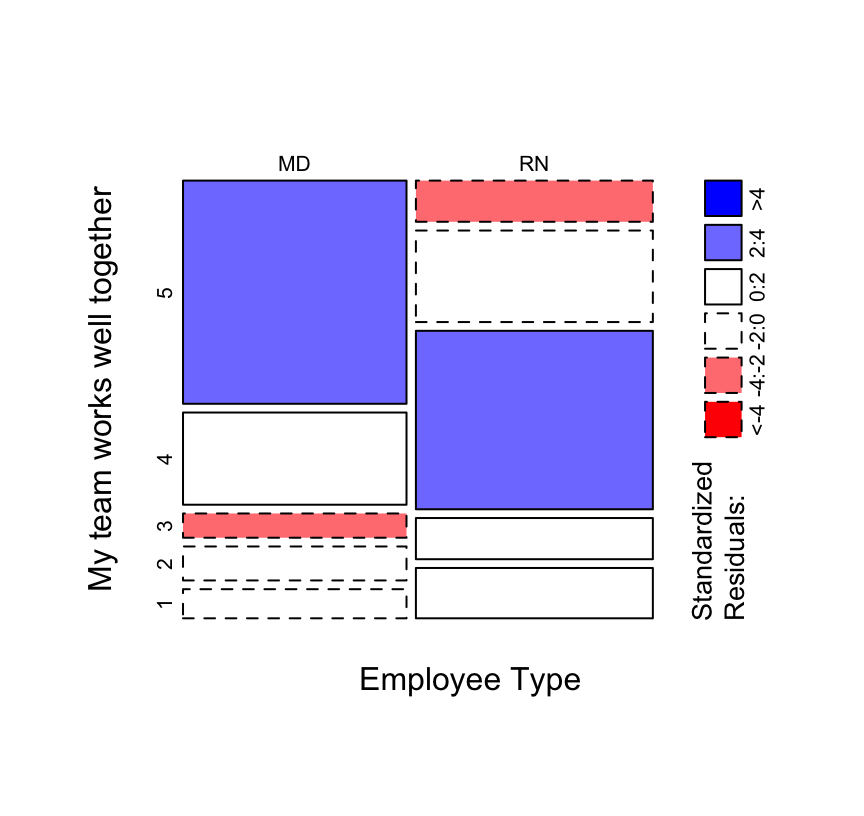
\includegraphics{likert_files/figure-latex/chisq-1} \end{center}

\begin{Shaded}
\begin{Highlighting}[]
\CommentTok{# Chi-square test}
\KeywordTok{chisq.test}\NormalTok{(both2_tab)}
\end{Highlighting}
\end{Shaded}

\begin{verbatim}
>  
>   Pearson's Chi-squared test
>  
>  data:  both2_tab
>  X-squared = 52.809, df = 4, p-value = 9.344e-11
\end{verbatim}

\hypertarget{Advanced}{\section{Multinomial regression}\label{Advanced}}

The multinomial regression model is a more powerful (and more modern)
version of the \(\chi^2\) test. Here, we're using an AIC-based
information-theoretic approach to determine whether the data as we see
it is as likely a model as a model that suggests no difference between
MD and RN responses. The probabilities can be plotted with a line chart
for easy comparison.

\emph{Multinomial regression between Employee Type and responses to the
`My team works well together' question, with information-theoretic table
for multi-model inference.}

\begin{Shaded}
\begin{Highlighting}[]
\CommentTok{# Multinomial regression}
\NormalTok{multnom_both =}\StringTok{ }\KeywordTok{multinom}\NormalTok{(Teamwork ~}\StringTok{ }\NormalTok{EmployeeType, }\DataTypeTok{data =} \NormalTok{both3, }\DataTypeTok{trace =} \OtherTok{FALSE}\NormalTok{)}
\NormalTok{multnom_both_1 =}\StringTok{ }\KeywordTok{multinom}\NormalTok{(Teamwork ~}\StringTok{ }\DecValTok{1}\NormalTok{, }\DataTypeTok{data =} \NormalTok{both3, }\DataTypeTok{trace =} \OtherTok{FALSE}\NormalTok{)}

\CommentTok{# New data for prediction}
\NormalTok{df_both =}\StringTok{ }\KeywordTok{data.frame}\NormalTok{(}\DataTypeTok{EmployeeType =} \KeywordTok{rep}\NormalTok{(}\KeywordTok{c}\NormalTok{(}\StringTok{"MD"}\NormalTok{, }\StringTok{"RN"}\NormalTok{), }\DataTypeTok{each =} \DecValTok{5}\NormalTok{),  }
  \DataTypeTok{Teamwork =} \KeywordTok{rep}\NormalTok{(}\KeywordTok{c}\NormalTok{(}\DecValTok{1}\NormalTok{:}\DecValTok{5}\NormalTok{), }\DecValTok{2}\NormalTok{))}

\CommentTok{# Get probabilities}
\NormalTok{multnom_both_probs =}\StringTok{ }\KeywordTok{cbind}\NormalTok{(df_both, }\KeywordTok{predict}\NormalTok{(multnom_both, }
  \DataTypeTok{newdata =} \NormalTok{df_both, }\DataTypeTok{type =} \StringTok{"probs"}\NormalTok{, }\DataTypeTok{se =} \OtherTok{TRUE}\NormalTok{))}

\CommentTok{# Clean up, ugh}
\NormalTok{multnom_both_probs =}\StringTok{ }\NormalTok{multnom_both_probs[,-}\DecValTok{2}\NormalTok{]}
\NormalTok{multnom_both_probs =}\StringTok{ }\KeywordTok{unique}\NormalTok{(multnom_both_probs)}

\CommentTok{# Make data frame for ggplot, probably should figure out tidyr}
\NormalTok{multnom_both_probs_df =}\StringTok{ }\NormalTok{reshape2::}\KeywordTok{melt}\NormalTok{(multnom_both_probs, }
  \DataTypeTok{id.vars =} \StringTok{"EmployeeType"}\NormalTok{, }\DataTypeTok{variable.name =} \StringTok{"Teamwork"}\NormalTok{, }
  \DataTypeTok{value.name =} \StringTok{"probability"}\NormalTok{)}

\CommentTok{# Figure 12}
\KeywordTok{ggplot}\NormalTok{(multnom_both_probs_df, }\KeywordTok{aes}\NormalTok{(}\DataTypeTok{x =} \NormalTok{Teamwork, }\DataTypeTok{y =} \NormalTok{probability, }
    \DataTypeTok{color =} \NormalTok{EmployeeType, }\DataTypeTok{group =} \NormalTok{EmployeeType)) +}
\StringTok{  }\KeywordTok{geom_line}\NormalTok{() +}\StringTok{ }
\StringTok{  }\KeywordTok{geom_point}\NormalTok{() +}
\StringTok{  }\KeywordTok{xlab}\NormalTok{(}\StringTok{"My team works well together"}\NormalTok{)}
\end{Highlighting}
\end{Shaded}

\begin{center}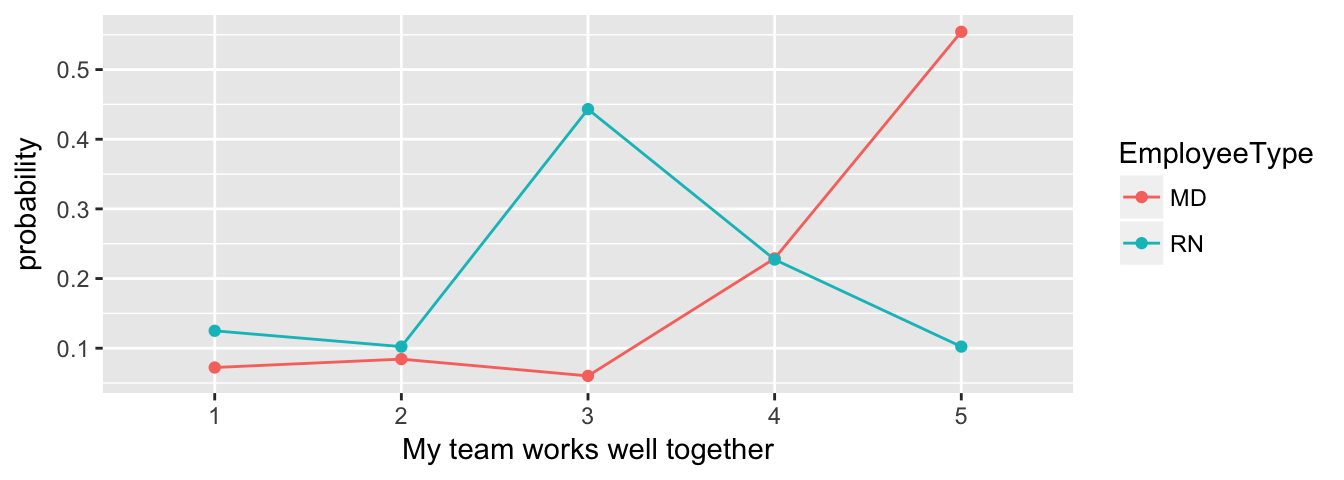
\includegraphics{likert_files/figure-latex/multnom-1} \end{center}

There appears to be an effect based on Employee Type; the AIC weight for
that model is practically 1, making it clearly the best model of the
model set.

\begin{Shaded}
\begin{Highlighting}[]
\CommentTok{# AICc table}
\NormalTok{mod_set =}\StringTok{ }\KeywordTok{list}\NormalTok{()}
    \NormalTok{mod_set[[}\DecValTok{1}\NormalTok{]] =}\StringTok{ }\NormalTok{multnom_both}
    \NormalTok{mod_set[[}\DecValTok{2}\NormalTok{]] =}\StringTok{ }\NormalTok{multnom_both_1}

\KeywordTok{kable}\NormalTok{(}\KeywordTok{aictab}\NormalTok{(mod_set, }\DataTypeTok{modnames =} \KeywordTok{c}\NormalTok{(}\StringTok{"Employee Type"}\NormalTok{, }\StringTok{"Null Model"}\NormalTok{)))}
\end{Highlighting}
\end{Shaded}

\begin{tabular}{l|r|r|r|r|r|r|r}
\hline
Modnames & K & AICc & Delta\_AICc & ModelLik & AICcWt & LL & Cum.Wt\\
\hline
Employee Type & 8 & 472.0249 & 0.00000 & 1 & 1 & -227.5680 & 1\\
\hline
Null Model & 4 & 522.0647 & 50.03976 & 0 & 0 & -256.9118 & 1\\
\hline
\end{tabular}

\section{Proportional-odds
regression}\label{proportional-odds-regression}

If you can meet the assumptions, the proportional-odds regression is
more powerful than the multinomial model, as it can take into account
the ordered nature of the ordinal scale.

Again, we use the information-theoretic approach to determine whether
there is an effect based on Employee Type, again plotted with a line
chart for easy comparison. And again the AICc results suggest an effect
is present. The probabilities are slightly different from the
multinomial model, but may be more accurate since we are now accounting
for the ordered nature of the response values.

\emph{Proportional odds regression between Employee Type and responses
to the `My team works well together' question, with
information-theoretic table for multi-model inference.}

\begin{Shaded}
\begin{Highlighting}[]
\CommentTok{# Proportional odds regression with polr}
\NormalTok{polr_both =}\StringTok{ }\KeywordTok{polr}\NormalTok{(Teamwork ~}\StringTok{ }\NormalTok{EmployeeType, }\DataTypeTok{data =} \NormalTok{Teamwork_tab_long, }
  \DataTypeTok{weight =} \NormalTok{Count)}

\CommentTok{# New data for prediction, same as multinom}
\NormalTok{df_both =}\StringTok{ }\KeywordTok{data.frame}\NormalTok{(}\DataTypeTok{EmployeeType =} \KeywordTok{rep}\NormalTok{(}\KeywordTok{c}\NormalTok{(}\StringTok{"MD"}\NormalTok{, }\StringTok{"RN"}\NormalTok{), }\DataTypeTok{each =} \DecValTok{5}\NormalTok{),  }
  \DataTypeTok{Teamwork =} \KeywordTok{rep}\NormalTok{(}\KeywordTok{c}\NormalTok{(}\DecValTok{1}\NormalTok{:}\DecValTok{5}\NormalTok{), }\DecValTok{2}\NormalTok{))}

\CommentTok{# Get probabilities}
\NormalTok{polr_both_probs =}\StringTok{ }\KeywordTok{cbind}\NormalTok{(df_both, }\KeywordTok{predict}\NormalTok{(polr_both, }\DataTypeTok{newdata =} \NormalTok{df_both, }
  \DataTypeTok{type =} \StringTok{"probs"}\NormalTok{, }\DataTypeTok{se =} \OtherTok{TRUE}\NormalTok{))}

\CommentTok{# Clean up, ugh}
\NormalTok{polr_both_probs =}\StringTok{ }\NormalTok{polr_both_probs[,-}\DecValTok{2}\NormalTok{]}
\NormalTok{polr_both_probs =}\StringTok{ }\KeywordTok{unique}\NormalTok{(polr_both_probs)}

\CommentTok{# Make data frame for ggplot, probably should figure out tidyr}
\NormalTok{polr_both_probs_df =}\StringTok{ }\NormalTok{reshape2::}\KeywordTok{melt}\NormalTok{(polr_both_probs, }\DataTypeTok{id.vars =} \StringTok{"EmployeeType"}\NormalTok{, }
  \DataTypeTok{variable.name =} \StringTok{"Teamwork"}\NormalTok{, }\DataTypeTok{value.name =} \StringTok{"probability"}\NormalTok{)}

\CommentTok{# Figure 13}
\KeywordTok{ggplot}\NormalTok{(polr_both_probs_df, }\KeywordTok{aes}\NormalTok{(}\DataTypeTok{x =} \NormalTok{Teamwork, }\DataTypeTok{y =} \NormalTok{probability, }
    \DataTypeTok{color =} \NormalTok{EmployeeType, }\DataTypeTok{group =} \NormalTok{EmployeeType)) +}
\StringTok{  }\KeywordTok{geom_line}\NormalTok{() +}\StringTok{ }
\StringTok{  }\KeywordTok{geom_point}\NormalTok{() +}
\StringTok{  }\KeywordTok{xlab}\NormalTok{(}\StringTok{"My team works well together"}\NormalTok{)}
\end{Highlighting}
\end{Shaded}

\begin{center}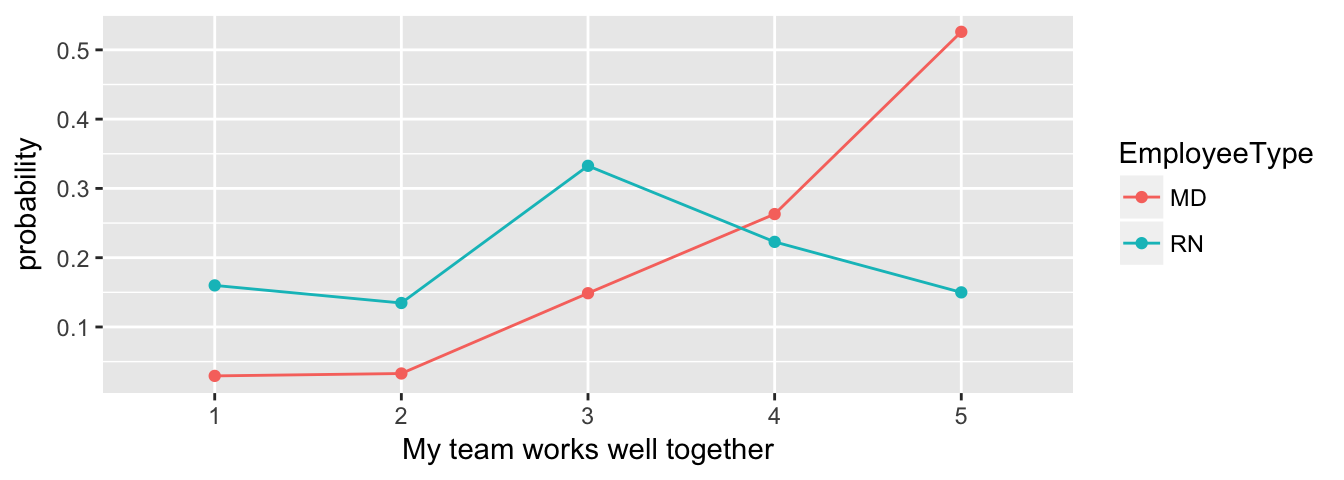
\includegraphics{likert_files/figure-latex/prop_odds-1} \end{center}

\begin{Shaded}
\begin{Highlighting}[]
\CommentTok{# I need to better understand diffs between polr and clm}
\CommentTok{# because polr objects don't play well with the AICcmodavg package}
\CommentTok{# Coefs/thresholds are exactly the same, though}
\NormalTok{fm1 =}\StringTok{ }\KeywordTok{clm}\NormalTok{(Teamwork ~}\StringTok{ }\NormalTok{EmployeeType, }\DataTypeTok{data=}\NormalTok{tab_df)}
\CommentTok{# Null model}
\NormalTok{fm2 =}\StringTok{ }\KeywordTok{clm}\NormalTok{(Teamwork ~}\StringTok{ }\DecValTok{1}\NormalTok{, }\DataTypeTok{data=}\NormalTok{tab_df)}

\CommentTok{# AICc table}
\NormalTok{mod_set =}\StringTok{ }\KeywordTok{list}\NormalTok{()}
    \NormalTok{mod_set[[}\DecValTok{1}\NormalTok{]] =}\StringTok{ }\NormalTok{fm1}
    \NormalTok{mod_set[[}\DecValTok{2}\NormalTok{]] =}\StringTok{ }\NormalTok{fm2}

\KeywordTok{kable}\NormalTok{(}\KeywordTok{aictab}\NormalTok{(mod_set, }\DataTypeTok{modnames =} \KeywordTok{c}\NormalTok{(}\StringTok{"Employee Type"}\NormalTok{, }\StringTok{"Null Model"}\NormalTok{)))}
\end{Highlighting}
\end{Shaded}

\begin{tabular}{l|r|r|r|r|r|r|r}
\hline
Modnames & K & AICc & Delta\_AICc & ModelLik & AICcWt & LL & Cum.Wt\\
\hline
Employee Type & 5 & 485.9008 & 0.00000 & 1 & 1 & -237.7686 & 1\\
\hline
Null Model & 4 & 522.0647 & 36.16387 & 0 & 0 & -256.9118 & 1\\
\hline
\end{tabular}

We can test the assumption of proportional odds with the \texttt{anova}
function. There's no evidence of a difference, suggesting that the
assumption is met.

\begin{Shaded}
\begin{Highlighting}[]
\NormalTok{fm3 =}\StringTok{ }\KeywordTok{clm}\NormalTok{(Teamwork ~}\StringTok{ }\NormalTok{EmployeeType, }\DataTypeTok{data=}\NormalTok{tab_df, }\DataTypeTok{threshold=}\StringTok{"equidistant"}\NormalTok{)}
\KeywordTok{anova}\NormalTok{(fm1, fm3)}
\end{Highlighting}
\end{Shaded}

\begin{verbatim}
>  Likelihood ratio tests of cumulative link models:
>   
>      formula:                link: threshold: 
>  fm3 Teamwork ~ EmployeeType logit equidistant
>  fm1 Teamwork ~ EmployeeType logit flexible   
>  
>      no.par    AIC  logLik LR.stat df Pr(>Chisq)
>  fm3      3 485.94 -239.97                      
>  fm1      5 485.54 -237.77   4.407  2     0.1104
\end{verbatim}

If the concepts or ideas in this section are confusing, it's probably
worth consulting a statistician for help evaluating your data with these
tools.

\chapter{A final word}\label{a-final-word}

``But everybody does it!'' \emph{Yeah, and they're wrong.}

``But it's directionally correct!'' \emph{When a concept is based on
discrete categories, ``in-between'' states are simply incoherent. The
light's either on or off, practically speaking.}

``But I want to!'' \emph{No. Just. No.}

\chapter*{Appendix: Measurement Levels \& Summary
Statistics}\label{appendix-measurement-levels-summary-statistics}
\addcontentsline{toc}{chapter}{Appendix: Measurement Levels \& Summary
Statistics}

\begin{longtable}[]{@{}lcccc@{}}
\toprule
\begin{minipage}[b]{0.25\columnwidth}\raggedright\strut
Statistic /\\
Parameter\strut
\end{minipage} & \begin{minipage}[b]{0.14\columnwidth}\centering\strut
Categorical\\
\emph{Nominal}\strut
\end{minipage} & \begin{minipage}[b]{0.11\columnwidth}\centering\strut
Ranked\\
\emph{Ordinal}\strut
\end{minipage} & \begin{minipage}[b]{0.18\columnwidth}\centering\strut
Discrete/Counts\\
\emph{Interval/Ratio}\strut
\end{minipage} & \begin{minipage}[b]{0.18\columnwidth}\centering\strut
Continuous\\
\emph{Interval/Ratio}\strut
\end{minipage}\tabularnewline
\midrule
\endhead
\begin{minipage}[t]{0.25\columnwidth}\raggedright\strut
Data set size (n)\\
Percent / Frequency\\
Count or rate\\
Categories (levels)\\
Mode\\
Median\\
Interquartile range\\
Median absolute deviation\\
Range\\
Minimum/maximum value\\
Quantiles\\
Mean (average)\\
Standard deviation\\
Coefficient of variation\\
\strut
\end{minipage} & \begin{minipage}[t]{0.14\columnwidth}\centering\strut
Y\\
Y\\
Y\\
Y\\
Y\\
\emph{No}\\
\emph{No}\\
\emph{No}\\
\emph{No}\\
\emph{No}\\
\emph{No}\\
\emph{No}\\
\emph{No}\\
\emph{No}\\
\strut
\end{minipage} & \begin{minipage}[t]{0.11\columnwidth}\centering\strut
Y\\
Y\\
Y\\
Y\\
Y\\
Y\\
Y\\
Y\\
Y\\
Y\\
Y\\
\emph{No}\\
\emph{No}\\
\emph{No}\\
\strut
\end{minipage} & \begin{minipage}[t]{0.18\columnwidth}\centering\strut
Y\\
Y\\
Y\\
Y\\
Y\\
Y\\
Y\\
Y\\
Y\\
Y\\
Y\\
Y\\
Y*\\
Y*\\
\strut
\end{minipage} & \begin{minipage}[t]{0.18\columnwidth}\centering\strut
Y\\
Y\\
Y\\
Y\\
Y\\
Y\\
Y\\
Y\\
Y\\
Y\\
Y\\
Y\\
Y*\\
Y*\\
\strut
\end{minipage}\tabularnewline
\bottomrule
\end{longtable}

* You must use the correct distribution (proper mean-variance
relationship) to ensure you get the correct standard deviation; most
software defaults to calculating the standard deviation for a
normally-distributed sample, which could be incorrect for certain kinds
of count, rate, or proportion data, for example.


\end{document}
